\documentclass[paper=a4,fontsize=11pt]{report}	% For KOMA, use scrartcl


% ------------------------------------------------------------------------------
% Imports and Packages
% ------------------------------------------------------------------------------
\usepackage[a4paper,includeheadfoot,margin=1in]{geometry} 	  % Document Formatting
\usepackage[english]{babel}                               	  % Typographical Rules
\usepackage[protrusion=true,expansion=true]{microtype}         % Typograhical Rules
\usepackage{amsmath,amsfonts,amsthm,amssymb} 			      % Non-native Math Symbols
\usepackage{float}                                             % For [H] centering
\usepackage{graphicx}                                          % For images
\usepackage[
		style=authoryear,
		citestyle=authoryear,
		sorting=nyvt,
		backend=biber,
		bibencoding=utf8,
		maxnames=2
		]{biblatex} % Citation
\usepackage{fancyhdr}                                          % Header customization

\usepackage{setspace}                                          % Double Spacing
\doublespacing 											      
															  % Table formatting
\usepackage{booktabs}
\usepackage[table,xcdraw]{xcolor}
\usepackage{longtable}

\usepackage{listings}                                          % Code Syntax Formatting and Highlighting
\usepackage{xcolor}                                            % Color Highlighting Rules
\usepackage[bottom]{footmisc}                                   % Fix footnotes to bottom


\addbibresource{references.bib}


% ------------------------------------------------------------------------------
% Listings Color Highlighting Rules
% ------------------------------------------------------------------------------
\definecolor{codegreen}{rgb}{0,0.6,0}
\definecolor{codegray}{rgb}{0.5,0.5,0.5}
\definecolor{codepurple}{rgb}{0.58,0,0.82}
\definecolor{backcolour}{rgb}{0.95,0.95,0.92}

\lstdefinestyle{mystyle}{
    backgroundcolor=\color{backcolour},   
    commentstyle=\color{codegreen},
    keywordstyle=\color{red},
    numberstyle=\tiny\color{codegray},
    stringstyle=\color{codepurple},
    basicstyle=\ttfamily\footnotesize,
    breakatwhitespace=false,         
    breaklines=true,                 
    captionpos=b,                    
    keepspaces=true,                 
    numbers=left,                    
    numbersep=5pt,                  
    showspaces=false,                
    showstringspaces=false,
    showtabs=false,                  
    tabsize=2,
    emph={
    to, 
    function,
    let, 
    in, 
    define, 
    add, 
    at, 
    as, 
    with, 
    parameters, 
    integer, 
    float, 
    string, 
    sort, 
    ascending, 
    descending,
    break,
    true,
    false,
    continue,
    next,
    loop,
    all,
    given,
    from,
    index
    },
    emphstyle={\color{red}}
}

\lstset{style=mystyle}


% Chapter Title Whitespace Modifier
\usepackage{titlesec}
\titleformat{\chapter}[display]   
{\normalfont\huge\bfseries}{\chaptertitlename\ \thechapter}{1em}{\Huge}   
\titlespacing*{\chapter}{0pt}{-50pt}{40pt}


% ------------------------------------------------------------------------------
% Definitions (do not change this)
% ------------------------------------------------------------------------------

\newcommand{\HRule}[1]{\rule{\linewidth}{#1}} 	% Horizontal rule

\makeatletter							        % Title
\def\printtitle{%						
    {\centering \@title\par}}
\makeatother									

\makeatletter							   
\def\printauthor{%					
    {\centering \large \@author}}				
\makeatother					


% ------------------------------------------------------------------------------
% LaTeX Variables and Shortcuts
% ------------------------------------------------------------------------------
\graphicspath{{../images/}}                      % Image Sources
\renewcommand*{\bibfont}{\small}                 % Make references text size small
\newcommand{\me}{Sahil Manojkumar Pattni}        % Author Name
\newcommand{\algo}{CGRG}
\newcommand{\setA}{\{A\}}
\newcommand{\setB}{\{B\}}
\newcommand{\abrule}{\setA\rightarrow\setB}

\newcommand{\pcite}[1]{\textbf{\parencite{#1}}}

%\DeclareNameAlias{sortname}{last-first}
% ------------------------------------------------------------------------------
% Metadata (Change this)
% ------------------------------------------------------------------------------


\title{	\normalsize \textsc{Final Year Dissertation} 	% Subtitle
		 	\\[2.0cm]								% 2cm spacing
			\HRule{0.5pt} \\						% Upper rule
			\LARGE \textbf{{Market Basket Analysis with Graph Theory}}	% Title
			\HRule{2pt} \\ [0.5cm]		% Lower rule + 0.5cm spacing
			\normalsize \today			% Todays date
		}



\author{
		Sahil M. Pattni\\	
		Bachelor of Science with Honours in Computer Science\\
        Supervised by Dr. Neamat El Gayar \\
}


\begin{document}
% ------------------------------------------------------------------------------
% Maketitle
% ------------------------------------------------------------------------------
\thispagestyle{empty}		% Remove page numbering on this page

\begin{figure}[H]
\centering

\includegraphics[scale=0.22]{hw_logo.png}
\end{figure}

\printtitle					% Print the title data as defined above
  	\vfill


\printauthor				% Print the author data as defined above

% ------------------------------------------------------------------------------
% Begin document
% ------------------------------------------------------------------------------
\pagebreak
\thispagestyle{empty}		% Remove page numbering on this page
\hspace{0pt}
\vfill
\section*{Declaration}
I, \me, confirm that this work submitted for assessment is my own and is expressed in my own words. Any uses made within it of the works of other authors in any form (e.g., ideas, equations, figures, text, tables, programs) are properly acknowledged at any point of their use. A list of the references employed is included.
\\\\Date: \today
\\Signed: \me

\vfill
\hspace{0pt}
\pagebreak

\newpage
\thispagestyle{empty}
\section*{Abstract}
In this digital age, data is being generated and collected at an unprecedented rate; data analytics is employed by corporations and small businesses alike to produce actionable insights and increase revenue.
Association rules allow us to identify relationships between products that can provide insights into customer spending habits and product perception.

Several algorithms exist for deriving association rules from transactional datasets, and many of these produce a vast number of rules, sometimes too many for the end-user to extract those that may ultimately be beneficial.
To that end, we introduce a novel algorithm: the \algo\ algorithm, that generates a limited number of high value association rules from a clustered minimum spanning tree, with each rule being of a distinct class: either a bi-cluster rule or an intra-cluster rule.
The quality of the generated rules was evaluated by using objective metrics such as support, confidence and lift.
The rules generated by our algorithm were compared against those generated by the Apriori Algorithm, and we observed that the ruleset generated by the \algo\ algorithm was primarily composed of only the high value rules present in the ruleset generated by the Apriori Algorithm.

% Table of Contents
\newpage
\setcounter{page}{1}
\pagenumbering{roman}
\tableofcontents
\newpage

\setcounter{page}{1}		% Set page numbering to begin on this page
\pagenumbering{arabic}

% Header settings
\pagestyle{fancy}
\fancyhf{}
\rhead{Page \thepage}
\lhead{\leftmark}
%\rfoot{Page \thepage}

% ------------------------------------------------------------------------------
% Chapters
% ------------------------------------------------------------------------------

\chapter{Introduction}


\section{Motivation}
For businesses such as groceries, hypermarkets, and retail outlets that deal with the trade of heterogeneous physical assets, operations such as inventory management and product placement play an instrumental role in determining the business' financial success. These involve asking questions such as:
\begin{itemize}
\item Which products should be placed at the entrance of the store? Which should be placed closer to the exit?
\item Which products will benefit the most by being placed at eye-level?
\item Which products should be placed next to each other to maximize the purchase volume?
\end{itemize}
One way to find optimal solutions to such queries is to employ the use of Association Rule Mining (also known as Market Basket Analysis). This set of techniques assess frequent itemsets (e.g. from sales data) and generate association rules between products. 
A prime example of the utility of association rules is the urban legend of \textit{"Beers and Pampers"}, where a company allegedly studied their point-of-sale data and found a strong association between the purchase of diapers and a particular brand of beer during certain days of the week. With \textit{diapers} as the antecedent and \textit{beer} as the consequent, this rule can be written as:
\[
\{\textit{Diapers}\} \rightarrow \{\textit{Beer}\}
\]
This is an example of a single-element rule, where both the antecedent and consequent are sets that contain only one element each. Several algorithms exist for association rule mining, most prominently the Apriori Algorithm \pcite{apriori} and FP-Growth \pcite{fp_growth}, however these algorithms tend to generate an overwhelming amount of rules, rendering it inconvenient for the end-user to extract actionable information from the ruleset.

\section{Aims}
%The aim of this project is to improve upon the aforementioned method by introducing a method that allows for the generation of multi-element association rules (i.e. rules where either/both the antecedent and consequent of the rule contain more than one element).
The aim of this project is to improve upon the methodology proposed by \pcite{mst_paper}, where the authors derived association rules from a minimum spanning tree. We plan on improving upon this by introducing a methodology to derive two distinctive types of rules (bi-cluster and intra-cluster) from a minimum spanning tree that has been segmented by a clustering algorithm.

\section{Objectives}
The research objectives for this paper are as described below:
\begin{enumerate}
\item Acquire a suitable dataset upon which the study can be conducted.
\item Construct an affinity graph from the chosen dataset.
\item Explore and evaluate MST extraction algorithms.
\item Explore methods for clustering topological structures such as graphs.
\item Extract the minimum spanning tree from the affinity graph.
\item Segment the minimum spanning tree into distinct clusters.
\item Develop and implement a methodology for extracting association rules from a clustered minimum spanning tree.
\item Evaluate the generated association rules against the rules generated by the Apriori Algorithm.
\end{enumerate} % Introduction
\chapter{Background}

\section{Transaction and Association Representation}
\subsection{Binary Purchase Vectors}
\label{sec:binary_purchase_vectors}
Let $I = I_1, I_2,\dots,I_m$ be a set of binary attributes (i.e. items), and let $T$ be a database of transactions.
As defined in \pcite{mine}, a binary purchase vector is a transaction $t$ represented as a vector of length $m$, where:
\[
t[k] = 
\begin{cases}
1 & \text{if } I_k \text{ purchased in } t\\
0 & \text{otherwise}\\
\end{cases}
\]
For example, consider a grocer who only sells five items: milk, eggs, bread, apples and oranges.
Consider the following transactions:
\begin{description}
\item[Transaction $t_1$:] Customer purchases bread and oranges.
\item[Transcation $t_2$:] Customer purchases eggs, bread and apples.
\item[Transaction $t_3$:] Customer purchases milk and oranges.
\end{description}
The binary purchase vectors for these transactions would be:
\begin{table}[H]
\centering
\begin{tabular}{@{}cccccc@{}}

\toprule
 & milk & eggs & bread & apples & oranges \\ \midrule
$t_1$ &  0    & 0    & 1     & 0      & 1       \\ \bottomrule
$t_2$ &  0    & 1    & 1     & 1      & 0       \\ \bottomrule
$t_3$ &  1    & 0    & 0     & 0      & 1       \\ \bottomrule
\end{tabular}
\caption{Binary Purchase Vectors}
\label{tab:binary_vectors}
\end{table}
\section{Product Association}
The association between products pairs across all transactions can be ascertained from the binary purchase vectors using the Pearson's Correlation Coefficient \pcite{pearson}. Since the correlations are of two binary variables, the Pearson's Correlation Coefficient is equivalent to the Phi-Coefficient $\phi$ \pcite{phi}, where for $n$ observations:
\[
\phi = \sqrt{\frac{\chi^2}{n}}
\]
Applying this correlation formula to the set of binary purchase vectors in Table \ref{tab:binary_vectors}, we get:
\begin{table}[H]
\centering
\begin{tabular}{@{}r|ccccc@{}}
\toprule
 & milk & eggs & bread & apples & oranges \\ \midrule
milk &   1.0    & -0.5    & -1.0     & -0.5      & 0.5       \\ \bottomrule
eggs &   -0.5    & 1.0    & 0.5     & 1.0      & -1.0       \\ \bottomrule
bread &  -1.0    & 0.5    & 1.0     & 0.5      & -0.5       \\ \bottomrule
apples & -0.5    & 1.0    & 0.5     & 1.0     & -1.0      \\ \bottomrule
oranges& 0.5    & -1.0    & -0.5     & -1.0      & 1.0      \\ \bottomrule
\end{tabular}
\caption{Correlation Matrix}
\label{tab:correlation}
\end{table}
\noindent Note that the correlation matrix is diagonally symmetrical. This is true of all correlation matrices where the items on the x-axis and y-axis are the same and in the same order. This correlation matrix can then be represented as a graph, where the nodes are the products, and the edges are the correlation values.

\section{Graph Theory}
\begin{figure}[H]
\centering
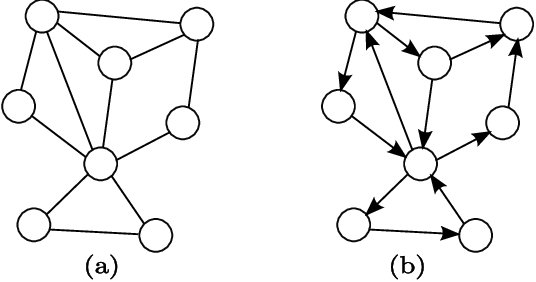
\includegraphics[scale=1.5]{graph-example}
\caption{Undirected and Directed Graphs}
\label{fig:graph.example}
\end{figure}
In discrete mathematics and more specifically - graph theory, a graph is a data structure that contains a set of nodes (i.e. vertices) connected by lines (i.e. edges).  These edges may be directed - such as in Figure \ref{fig:graph.example}:(a), or undirected - such as in Figure \ref{fig:graph.example}:(b). The edges may contain values (i.e. weights) between the two vertices it connects. A graph $G$ with a set of vertices $V$ and a set of edges $E$ can be represented via the notation $G = (V,E)$. For the scope of this project,  we will be building undirected graphs, where the weight between two vertices is the same in both directions.

\subsection{Minimum Spanning Trees}
Given an undirected $G = (V,E)$,  a \textit{spanning tree} can be described as a subgraph that is a tree which includes all the vertices $V$ of $G$ with the minimum number of edges required. A \textit{minimum spanning tree} (MST) is the spanning tree with the smallest sum of edge weights.  This means that if the graph has $n$ vertices, each spanning tree - including the minimum spanning tree - will have $n-1$ edges. Since a minimum spanning tree captures the lowest weights in a graph, with modifications it could be an excellent candidate to capture the opposite as well: the strongest associations between products.
There are two widely used algorithms to extract the minimum spanning tree from a graph: Prim's algorithm and Kruskal's algorithm.

\subsection{Prim's Algorithm}
Independently discovered by three authors,  Prim's algorithm \pcite{prims}\pcite{prims_og}\pcite{prims3} is a greedy algorithm\footnote{Selecting the locally optimal choice at each iteration of the solution} to find the minimum spanning tree of an undirected,  weighted graph $G$. To successfully implement the algorithm, three sets need to be maintained: a set of \textit{discovered} edges, and two sets of vertices: a set of \textit{undiscovered} vertices, and a set of \textit{discovered} vertices.  Figure \ref{fig:prim} illustrates Prim's algorithm being applied to a graph. The algorithm is as follows:\\
Initialize an empty set of discovered edges: $E$, and two sets of vertices: an empty set $D$ of the discovered vertices, and $UD$ as the set of undiscovered vertices.
\begin{itemize}
\item Pick an arbitrary vertex as a starting point (in the case of Figure \ref{fig:prim}, the top right node). Add this vertex to $D$ and remove it from $UD$.
\item While $UD$ is not empty:
	\begin{itemize}
	\item Find the edge $e_i$ with the smallest weight such that it connects together a vertex $V_1$ in $D$ and $V_2$ in $UD$ (to avoid forming cycles).
	\item Append $V_2$ to $D$ and remove it from $UD$ (i.e. $V_2$ is now discovered).
	\item Append $e_i$ to $E$.
	\end{itemize}
\end{itemize}
Once $D$ contains all the vertices of $G$, the algorithm terminates, and the set $D$ represents the minimum spanning tree, and $\sum\limits_{i=1}^n e_i$ is the weight of the MST. The time complexity of this algorithm is $O(V^2)$.
\begin{figure}[H]
\centering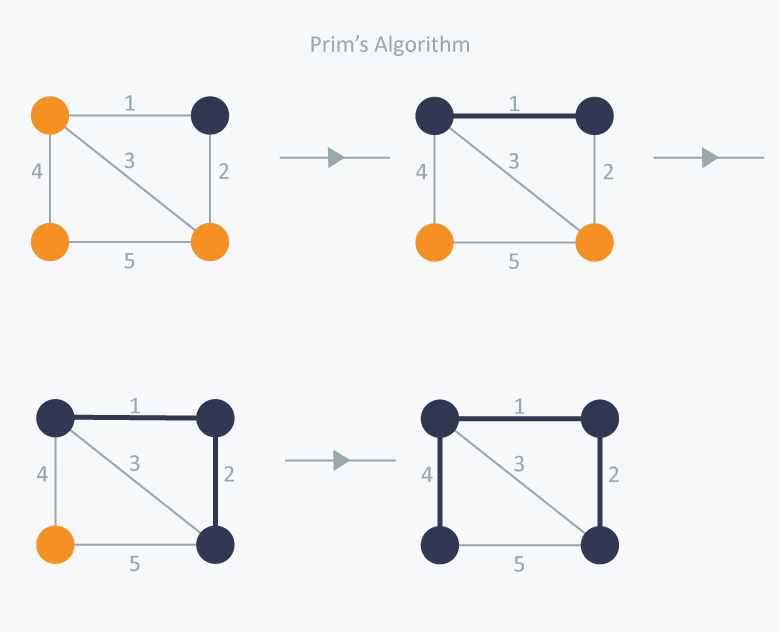
\includegraphics[scale=0.5]{prims}
\caption{Prim's Algorithm applied to a graph \pcite{prim-pic} }\label{fig:prim}
\end{figure}

\subsection{Kruskal's Algorithm}
Another greedy algorithm,  Kruskal's algorithm \pcite{kruskal} also extracts the MST from a graph.  Unlike Prim's algorithm, Kruskal's doesn't select an edge that connects directly to the already built spanning tree, but rather picks the global optimal solution. The algorithm is as follows:\\
Maintaining a set of edges $E$, and an initially empty set of chosen edges $C$:
\begin{itemize}
\item Sort the set of edges $E$ in ascending order.
\item While the number of elements in $C$ is not $n-1$:
	\begin{itemize}
	\item Select the smallest edge $e_i$ from $E$.
	\item If adding it does not form a cycle with the spanning tree formed so far, append $e_i$ to $C$.
	\item Remove $e_i$ from $E$.
	\end{itemize}
\end{itemize}
The algorithm will terminate when $n-1$ edges have been selected.  The time complexity for this algorithm is $O(ElogE)$.





\section{Related Work}

\subsection{Extracting Minimum Spanning Trees using K-Means}
\pcite{kmeans_mst} proposed a novel framework to extract the minimum spanning tree of a graph based on the K-Means clustering algorithm. Their methodology can be separated into two distinct phases. In the first phase,  the data is partitioned into $\sqrt{n}$ clusters via K-Means and the Kruskal's algorithm is applied to each of the clusters individually.  Once the $\sqrt{n}$ MSTs have been constructed, they are combined to form an approximate MST. In the second phase,  new partitions are constructed based on the borders of the clusters identified in phase 1.  Based on these new partitions, a second approximate MST is constructed.  Finally, both graphs are merged such that the resulting graph has $2(n-1)$ edges. The Kruskal's algorithm is run on this graph to get the final approximation of the MST.
\\\\\textbf{Critical Analysis}\\
The authors have proposed an efficient way to approximate a minimum spanning tree, with their methodology having a complexity of $O(N^{1.5})$, which is faster than the standard MST algorithm which has a complexity of $O(N^2)$. 
For clarity, we have illustrated the disparity between the author's algorithm and the standard algorithm on Figure \ref{fig:speed-compare}.
\begin{figure}[H]
\centering
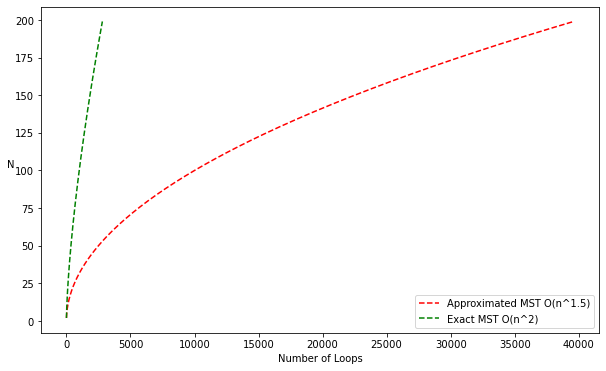
\includegraphics[scale=0.6]{speed-compare} 
\caption{Efficiency of K-Means optimized MST vs.  exact MST}\label{fig:speed-compare}
\end{figure}
\noindent  The K-Means optimized algorithm is $\frac{\sqrt{n}-1}{\sqrt{n}}\%$  faster than the standard MST algorithm.


\subsection{Markov Clustering}
\pcite{markov_clustering} introduced the novel Markov Clustering Algorithm (MCL), a graph clustering algorithm based on Markov Processes \pcite{markov_original} that favours sparse graphs (i.e. graphs where the average degree is smaller than the number of nodes). 
The reason for this follows the notion that dense regions in sparse graphs correspond with regions in which the number of $k$-length paths is relatively large - and therefore - paths whose beginnings and ends are in the same dense region have a higher probability for random walks\footnote{A random walk is a stochastic process of of successively random steps along a space, in this case: a directed graph.} of length $k$ as opposed to other paths.
In other words, random walks originating from a node in a dense region have a high probability of ending in that same dense region.
Given a non-negative weighted directional graph $G$, the MCL simulates flow in the graph. 
It does this by first mapping the graph $G$ in a generic way onto a Markov matrix $M_1$.
Once completed, the set of transition probabilities (TP's) are iteratively recomputed via expansion and contraction, resulting in an array of Markov Graphs.
In the expansion stage, higher TP's are calculated, whereas for the contraction phase, a new Markov Graph is created by rewarding high TP's and penalizing low TP's.
The belief is that by doing so, the flow between dense regions that are sparsely connected will be removed, leaving only distinct and unconnected dense regions (i.e. clusters).
The author tested the MCL algorithm against randomly generated graphs which were known to possess a natural cluster structure. The authors noted that the MCL algorithm successfully managed to capture the segregation present in the graphs, and concluded that the algorithm was capable of handling graphs with large natural clusters.
\\\\\textbf{Critical Analysis}\\
The author proposed a novel way to apply the mathematics behind Markov processes to successfully segment and isolate densely connected segments of a graph. The results from this paper have inspired us to use the clustering algorithm in our own work.


\subsection{AIS Algorithm}
\label{sec:ais}
\pcite{mine} proposed a novel algorithm to generate all statistically significant association rules between items in a database, laying the foundation for association rule mining. Given a set of items $I = \{I_1, I_2, I_3,\dots,I_m\}$, the authors define an association rule to be of the form $X \rightarrow I_j$ where X is a set of items such that $X \subset I, I_j \notin X$.  The hypothetical database stated was a list of transactions, $T$, where each transaction $t$ was a binary vector of length $m$, as described in Section \ref{sec:binary_purchase_vectors}. The authors define two constraints for assessing association rules:
\\\\\textbf{Support}\\
The support of an association rule is the proportion of transactions in which the itemsets in the rule are present. For a set of transactions $T$, where $T(i)$ denotes the set of transactions in which the set of items $i \subseteq I$ was purchased:
\[
\text{support}(i) = \frac{T(i)}{T} 
\]
Similarly, where $T{(i_k, i_j)}$ represents the set of transactions in which the itemsets $\{i_k \subset I, i_j\subset I\}$ were purchased, the support for the association rule $i_k \rightarrow i_j$ can be represented as:
\[
\text{support}(i_k \rightarrow i_j) = \frac{T(i_k, i_j)}{T} 
\]
Support scores correspond with the statistical significance of a rule, and rules with low support scores may not occur frequently enough to draw reasonable conclusions from.
\\\\\textbf{Confidence}\\
Confidence is the conditional probability of an itemset $i_j;\;\;i_j \subset I$ being present in a transaction given that itemset $i_k;\;\;i_k \subset I$ is present in the same transaction. The confidence of the association rule $i_k \rightarrow i_j$ can be represented as:
\[
\text{confidence}(i_k \rightarrow i_j) = \frac{T(i_k, i_j)}{T(i_k)} \equiv \frac{\text{support}(i_k \rightarrow i_j)}{\text{support}(i_k)}
\]
The confidence of an association rule can be thought of as the rule's \textit{strength}.
\\With these constraints defined, the authors state that their methodology for association rule mining can be split into two discrete steps:
\begin{enumerate}
\item The generation of candidate itemsets.
\item The generation of statistically significant association rules from the itemsets.
\end{enumerate}
\textbf{Candidate Itemset Generation}\\
To generate candidate itemsets, the authors first generate all possible itemsets from the database, defining those whose support score was above a support constraint $\textit{min}_\textit{support}$ as \textit{large itemsets}. The authors note that a brute-force check\footnote{checking every possible itemset iteratively.} would be sub-optimal, taking up to $2^m$ passes of the database (where $m$ is the number of items in the itemset $I$). Therefore, they introduced a methodology where they would only observe itemsets of length $k$ on the $k^{th}$ pass of the dataset, to see if the itemsets satisfied the support constraint. On the $(k+1)^{th}$ pass of the dataset, they need only check itemsets that are \textit{1-extensions} (i.e. itemsets extended by only one item) or the \textit{large itemsets} discovered in the previous pass. Their reasoning is now commonly known as \textit{The Apriori Principle}, where they state that if an itemset $i_k$ is \textit{large} (i.e. satisfies the support constraint), then any subset $i_j \subset i_k$ will also be \textit{large}. This reasoning also applies that if an itemset $i_j$ is found to be \textit{small} (i.e. did not satisfy the support constraint), then any superset $i_k; i_j \subset i_k$ will also be \textit{small}. This allows the authors to prune the number of association rules whose support scores need to be computed, as if they find $i_j$ to be \textit{small}, any superset $i_k; i_j \subset i_k$ need not have its support score computed as it is known to be \textit{small}.\\
However, if an itemset $i_j$ is indeed found to be \textit{large}, then another multiple passes over the dataset will be required to check the support scores for subsets of $i_j$. To avoid this, the authors devised a measure to calculate the expected support $\bar{s}$ of an itemset. The expected support is used to estimate the support of $i_j = (i_p + i_q)$, not only when $i_j$ is expected to be \textit{large}, but also when $i_p$ is expected to be \textit{large} yet $(i_p + i_q)$ is expected to be \textit{small}. This estimation further prunes the number of rules whose support scores need to be computed.
\\\\\textbf{Association Rule Generation}\\
To generate association rules, the authors used the following technique:\\
for each \textit{large} itemset $Y = \{i_1, i_2,\dots,i_k\}; k \geq 2$ from the set of non-pruned \textit{large} itemsets, generate a set of association rules in the form $X \rightarrow i_j; X \subset Y, i_j \notin X$ such that $X$ is of length $k-1$. Therefore, each \textit{large} itemset will produce $k$ rules. From the generated rules, the authors discarded those rules whose confidence scores fell below the confidence constraint $\textit{min}_\textit{confidence}$.
\\\\\textbf{Evaluation}\\
The authors tested their methodology on a sales dataset with $46,783$ transactions, with $63$ distinct departments. Their configuration was composed of a support constraint of $1\%$ (i.e. $\textit{min}_\textit{support} = 0.01$) and a confidence constraint of $50\%$ (i.e. $\textit{min}_\textit{confidence} = 0.5$). The authors note that the rules produced follow what general intuition might suggest. For example:
\[
\{\text{Auto Accessories, Tires}\} \rightarrow \{\text{Automotive Services}\}
\]
Furthermore, the authors assessed the accuracy of their support estimation metric $\bar{s}$ by observing the ratio of correctly estimated itemsets for both \textit{small} and \textit{large} against various values for the support constraint. They were able to conclude that their estimation accuracy was satisfactory, as their accuracy was  $96\%$ and above for support thresholds.
\\\\\textbf{Critical Analysis}\\
The authors have proposed a novel methodology that has been the bedrock of numerous research publications,  including most of the papers in this literature review.  Their estimation function performed with high accuracy, meaning it can reduce the number of passes through a database the algorithm has to take by a significant amount. Additionally, their pruning techniques allowed them to eliminate a large proportion of itemsets from the space. Even after the significant pruning of rules, a major drawback of this methodology is the large number of rules produced, although one could argue that only the highest performing rules need be observed in further detail. Finally, the algorithm only allows the consequent to have one item, thereby limiting the type and quality of rules produced.

\subsection{Apriori Algorithm}
\label{sec:apriori}
\pcite{apriori} improved on their previous work with \pcite{mine} by introducing the Apriori algorithm, which - in addition to being faster than the AIS algorithm - can produce association rules where the consequent has more than one item. The structure for the Apriori algorithm follows closely to to the AIS algorithm in that it uses \textit{large} itemsets to generate the association rules.
The algorithm generates candidate itemsets in the $k^{th}$ pass only from the itemsets found to be \textit{large} in the $(k-1)^{th}$ pass, following the intuition of \textit{The Apriori Principle}, where any subset of a \textit{large} itemset must itself be \textit{large}. As a result, the candidate itemsets that have $k$ items can be generated from the \textit{large} itemsets having $(k-1)$ itemsets, and any such itemsets that contain a subset that is \textit{small} are discarded.
For every \textit{large} itemset $l$, all non-empty subsets of $l$ are gathered. For every subset $a$, it generates a rule in the form:
\[ a \rightarrow (l-a) \]
if the support and confidence constraints of the rule are met.
\\\\\textbf{Critical Analysis}\\
The authors have further improved upon their AIS algorithm in the form of the Apriori Algorithm, which is much better known than the former due to its inherent ability to generate more complex rules, and its efficiency in doing so. The ability to generate more complex rules makes it a good benchmark to test our own algorithm against, to see whether it can either serve as an alternative or even a complement to the Apriori Algorithm.


\subsection{Subjective Measurement of Association Rules}
\pcite{market_ass} proposed a novel measure for the \textit{interestingness} of association rules,  identifying that a dominant, universally used measure did not exist. The authors' goal was to combine objective measures such as the support, confidence and lift scores with more subjective measures. Instead of the Apriori approach, their methodology has them generate association rules via the \textit{tree-building technique} - which compresses a large database into a Frequent-Pattern tree, citing that this technique was more efficient than the Apriori algorithm. The authors employed the heuristical unexpectedness measure\footnote{How significantly a rule contradicts a user's prior beliefs.} and the heuristical actionability measure\footnote{If the user believes they can use the information to their advantage (e.g. a promotion).} as their subjective measures, and a minimum confidence threshold of 51\% as their objective measure.  Since a subjective measure would require a human subject, the authors' used the estimations of a sales manager from a Croatian retail chain, and stored his responses in binary format for the subjective measures (i.e. 0 if a rule was unexpected else 1, 0 if a rule is not useful else 1). The dataset used for this paper was a real transactional dataset with 14,012 transactions and a set of 1,230 unique items (which was later pruned to 7,006 transactions and a set of 278 products) from the same Croatian retail chain their test subject worked at. The authors then generated association rules from the first-level hierarchical grouping of items from the dataset (items with a minimum support of 25\%),  of which 36 rules were identified as statistically significant.  From this set of rules, only two rules satisfied both subjective measures and the confidence constraint, and therefore these two rules were identified as highly interesting.  The authors then generated association rules from the second-level hierarchical grouping of items, where items that represented the same product (but had different a manufacturer, brand etc.) were grouped together. Of the rules generated, 15 satisfied their confidence constraints and had a support value able 10\%. 5 rules from this set satisfied both their subjective and objective measures,  more than the previous experiment  The authors were able to conclude that the increase in accuracy and number of interesting rules resulted from the second level of grouping which generalized the products.\\
\\\\\textbf{Critical Analysis}\\
Wheras the original measure of statistical significance introduced by \pcite{mine} was purely objective, the authors  of this paper have presented a well thought out approach to combining the subjective metrics with objective ones to produce a human-verified association rule set.  A few caveats to note, however: their study only involved one subject, which is rarely regarded to be statistically acceptable. An ideal study would require multiple, randomly chosen subjects to offset any bias that the singular subject would have had, and in addition, the larger their subject size, the closer their collective estimations will model the total population's.  Another drawback of their approach is that by using human intuition as a metric,  they're promoting association rules that satisfy pre-existing notions about human behavior (e.g. if someone buys milk, they'll \textit{probably} get eggs too), however these types of rules are usually regarded as common knowledge,  whereas the beauty of association rule mining is in its ability to surface association rules that - while true - seem unintuitive, and therefore are less likely to be known by the management of such organizations.


% MAIN MST PAPER
\subsection{Association Rules from Minimum Spanning Trees}
\label{sec:mst paper}
\pcite{mst_paper} proposed a novel methodology to study the structure and behavior of consumer market baskets from the topology of a minimum spanning tree which represented the interdependencies between products, and use this information to complement the association rule generation process. The input to their proposed methodology was a correlation matrix between the set of all binary purchase vectors for every transaction.  The dataset used for the MST construction was a list of $1,046,804$ transactions containing a set of $3,240$ unique products from a large supermarket chain branch in Santiago, Chile.  When building this correlation matrix, the authors opted to use the Pearson's Coefficient \pcite{pearson} - which is equivalent to the coefficient $\phi$ for binary data \pcite{phi} - over the traditionally used Jaccard distance to compute the similarity between the binary product vectors, as the former provides both a positive and negative association between products. Additionally,  they used the distance function $d_{ij} = \sqrt{2(1-\phi_{ij})}$ to transform the correlation matrix into a distance measurement (i.e. the weight of the edges)\footnote{$\phi_{ij}$ is the correlation score between products at indexes $i$ and $j$ on the correlation matrix.}. 
\\\\\textbf{MST Analysis}\\
The authors constructed a MST for 220 product subcategories, and noted that there was a significant level of grouping between product sub-categories that belonged to the same parent category.  To remove edges from the MST that were not statistically significant,  the authors used the mutual information \pcite{measure} measure $\sum\limits_{x,y}log_2 \frac{r(x,y)}{p(x)q(y)}$ between product subcategories $p$ and $q$, and were able to prune 14 edges, all of which were connected to a terminal node, therefore effectively pruning 14 vertices from the MST too. To identify the most influential regions of the MST, the authors defined an influence zone of distances that were in the $10^{th}$ percentile. To generate meaningful association rules,  for each MST product $i$, the authors ran a search for the set of all association rules $R_i$ such that $P_i \rightarrow P_j (i \neq q)$. Then from the resulting set of rules, they searched for rules that obeyed $P_i \rightarrow P_m$ where $m$ a product node connected to the product $i$ in the minimum spanning tree.  For both resulting sets of rules for each product, the mean of their lift scores were observed, and the authors determined that the rules that were reinforced by the MST had a higher mean, and that a majority of these rules had a lift score above the $90^{th}$ percentile. 
\\\\\textbf{Inherent Clustering}\\
To identify the clusters each of the products should be identified under, the authors constructed a hierarchical tree using the average linkage clustering method, and by using an unspecified cut distance, they were able to produce 17 taxonomic groups (i.e. clusters). Cross-referencing their results with the actual parent categories of the products, they were able to conclude that the MST did indeed categorize the product sub-categories into clusters with a reasonable degree of accuracy.
\\\\\textbf{Comparing to an alternative methodology}\\
The authors then compared their MST to another methodology, namely the structured association map (SAM) \pcite{kim}, using the Jaccard distance as a measure of similarity,  and were able to generate interesting 2x2 rules (i.e. $\{A,B\}\rightarrow\{C, D\}$), all with lift scores above 1.0, with one rule even having a lift score of 106.46. They concluded that while both approaches provided different information, they both visually identify the strongest relationships between the products, and provide useful information to reduce the search space for association rules.
\\\\\textbf{Critical Analysis}\\
The authors' approach seems to be novel,  thorough and well structured.  Their methodology successfully employed the use of minimum spanning trees to complement the association rule generation process with sound results.  One caveat of their approach is that they only used the MST to generate single-element rules (i.e. $\abrule$, where the antecedent and consequent contain only one element each). Using the distance score in conjunction with the importance function they defined (i.e. $\sum\limits_{k \in K_u}^{} \frac{1}{w_{uk}}$), they could have defined a system to produce multi-element rules (i.e. where either/both the antecedent and the consequent have more than one element) While single-element rules are easily understandable and tend to have high lift values when extracted from the MST, multi-element rules would provide an additional layer of insight as to how a range of products (perhaps a cluster) relate to another.


\subsection{Summary}
In conclusion, \pcite{mine} introduced a formal system for association rules, and a method to generate them from a transactional database, which was further improved when \pcite{apriori} introduced the Apriori Algorithm.
Instrumental to the success of this algorithm is its ability to prune a bulk of the rules such that their support scores need not be checked. \pcite{num_rules} defines the equation for calculating the number of possible rules for an itemset \textbf{\textit{d}} as:
\[
\textit{number of rules} = \sum\limits_{k=1}^{d-1} \left(\binom{d}{k} \times \sum\limits_{j=1}^{d-k}\binom{d-k}{j}  \right)
\]
\begin{figure}[H]
\centering
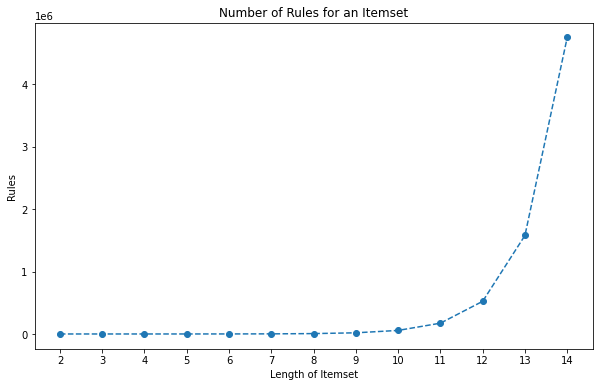
\includegraphics[scale=0.6]{numrules}
\caption{Number of Association Rules for an Itemset}
\label{fig:numrules}
\end{figure}
We have plotted Figure \ref{fig:numrules} to illustrate the exponential growth of rules given an itemset's length \textbf{\textit{d}}.
This exponential growth reinforces the need for the rule pruning techniques introduced in \pcite{mine} to be able to complete the computations within a reasonable time frame, and will therefore be incorporated into our methodology.
However, while these papers only based the interestingness of an association rule on objective measures such as the support, confidence and lift scores of these rules, \pcite{market_ass} proposed a methodology where subjective human input was used to validate the interestingness of these rules. A drawback of the above methods, however, is the large number of rules produced.
\pcite{kmeans_mst} proposed a solution to the relatively slow computation time that the Prims's algorithm and Kruskal's algorithm offer, where the Kruskal's algorithm was optimized using K-Means, leading to a significant performance increase as illustrated in Figure \ref{fig:speed-compare}. The methodology proposed in this paper was a framework, where Kruskal's Algorithm could be substituted with any MST algorithm, such as Prim's Algorithm.
\pcite{markov_clustering} introduced a novel way to identify and isolate dense regions within a graph, and we have used their algorithm to cluster our own graphs.
\pcite{mst_paper} introduced a methodology to extract high value association rules from a minimum spanning tree, used to complement the rules produced by the Apriori algorithm. A caveat of this approach, however, is that it can only produce rules such that the antecedent and consequent are sets with one element each. This paper has been the primary motivation for our work, and therefore we have incorporated into our work several techniques that the authors used and/or introduced.
\\As a note, \pcite{lift} defined another metric to assess association rules - \textit{conviction} - now commonly referred to as \textit{lift}. The lift of an association rule $i_k \rightarrow i_j$ is the rise that $i_k$ gives to the confidence of the rule. The formula for lift is:
\[
\text{lift}(i_k \rightarrow i_j) = \frac{\text{confidence}(i_k \rightarrow i_j)}{\text{support}(i_j)}
\] 
All the research conducted above has served as the inspiration for this project.
   % Background

\chapter{The \algo\ Algorithm}
In this section, we introduce the main contribution of this paper: the Clustered-Graph Rule Generation (CGRG) algorithm. The \algo\ algorithm derives association rules from a clustered minimum spanning tree. This chapter will focus on the workings of the algorithm.

\section{Data Processing}
\label{sec:algo_data}
Given an itemset $I = \{I_1, I_2,\dots,I_m\}$ and a set of tranactions $T = \{T_1,T_2,\dots\,T_n\}$ such that $T_i \subseteq I$, every transaction $T_i$ will be transformed into a binary purchase vector, as described in Section \ref{sec:binary_purchase_vectors}. An $m \times m$ correlation matrix will then be computed using the Pearson's Correlation Coefficient from the set of binary purchase vectors, composed of the correlation every item has against every other item. A graph $G = (V,E)$ will be constructed from this correlation matrix, such that the vertices $V=I$, and every edge will be the correlation value between the two items it connects. A minimum spanning tree is a sub-graph composed of the \textit{shortest} path connecting all vertices (i.e. the lowest sum of weights), and therefore if we construct our graph from the correlation matrix, the MST would only capture strongly negative and weakly positive relationships only, whereas we want to capture the strongest relationships between products. Therefore to extract a MST with the strongest associations, the values in the correlation matrix must first be transformed before a graph is constructed from them.

\section{Distance Function}
\label{sec:distance}
As mentioned in Section \ref{sec:binary_purchase_vectors}, the Pearson's Correlation Coefficient is equivalent to the Phi Coefficient ($\phi$) for binary variables, as is the case for our binary purchase vectors. Given $\phi_{ij}$ for items $I_i$ and $I_j$ in the correlation matrix, \pcite{mst_paper} used the distance function
\[
\phi_{ij} = \sqrt{2(1-\phi_{ij})}
\]
to transform their correlation matrix. Given that we are using the Pearson's Correlation Coefficient that gives us a correlation score in the interval [-1,1], this equation is not suitable for us as it discards the strongly negative associations by outputting a larger weight (e.g. a correlation score of -1 would be transformed to 2) which would not be captured in the MST. Therefore, we modify the equation to be
\[
\phi_{ij} = \sqrt{2(1-|\phi_{ij}|)}
\]
allowing us to capture both positive and negative associations alike. Figure \ref{fig:distance_function} illustrates the effect of our distance function, where the stronger the correlation of the input, the lower the output. Given that our initial correlation values were bound to the interval $[-1,1]$, the output of the distance function is similarly bound to the interval $[0, \sqrt{2}]$.
\begin{figure}[H]
\centering
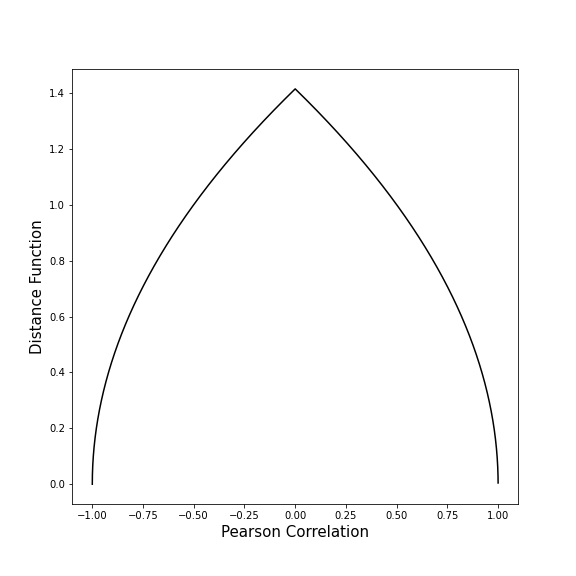
\includegraphics[scale=0.4]{distance_function}
\label{fig:distance_function}
\caption{The effect of the distance function $\sqrt{2(1-|x|)}$}
\end{figure}
\noindent Once the correlation matrix has been transformed via this function, the graph $G=(V,E)$ can be constructed. Using Kruskal's algorithm, the minimum spanning tree can then be constructed from the graph $G$.

\section{Clustering and Rule Generation}
\subsection{Markov Clustering}
Once the MST has been constructed, it can then be clustered using the Markov Clustering (MCL) Algorithm. Multiple cluster configurations will be generated using the algorithm with varying inflation scores to identify the most modular configuration\footnote{Where the connectedness between dense clusters is minimal}, which will then be used to segment the MST.

\subsection{Itemset Generation}
For every cluster $Cl_i$ identified by the MCL algorithm, all proper subsets $cl$ such that $cl \subseteq Cl_i$ are generated. The set of proper subsets are stored against the key $i$, which denotes the index of cluster $Cl_i$, effectively assigning each cluster its proper subsets. Listing \ref{lst:itemset_generation} is the pseudo-code for this operation.
\begin{lstlisting}[language=C, mathescape=true, caption=Cluster Itemset Generation, label=lst:itemset_generation]
given CLUSTERS = {$Cl_1, Cl_2,\dots,Cl_n$}
define itemsets_by_cluster as {$\emptyset$}
for $Cl_i$ in CLUSTERS
    to items_by_cluster add ({all $cl$ if $cl \subseteq Cl_i$} at index $i$)
\end{lstlisting}

\subsection{Bi-Cluster Rule Generation}
Bi-cluster rules are those where the antecedent and the consequent originate from distinct and separate clusters. All possible bi-cluster rules are generated such that for any two given clusters $Cl_k$ and $Cl_j$:
\[
cl_k \rightarrow cl_j;\;\; cl_k \subset Cl_k, \; cl_j \subset Cl_j
\]
Listing \ref{lst:bicluster} presents the pseudo-code for the bi-cluster rule generation. All bi-cluster combinations are generated and stored as a pair of indices (i.e. $(i,j)$ for clusters $Cl_i$ and $Cl_j$). For every cluster pair generated, every configuration itemsets associated with each cluster (calculated in Listing \ref{lst:itemset_generation}) is added to the ruleset such that a rule exists for every itemset $c_k$ associated with cluster $C_k$ and every itemset $c_j$ associated with cluster $C_j$.

\begin{minipage}{\linewidth}
\begin{lstlisting}[language=C, mathescape=true, caption=Bi-Cluster Rule Generation, label=lst:bicluster]
given CLUSTERS = {$Cl_1, Cl_2,\dots,Cl_n$}
given itemsets_by_cluster = {$\dots$} // already populated
define rules as $\emptyset$
define combs as $\emptyset$
to combs add all $^nC_2$ combinations from {$1,2,\dots,n$}

for comb in combs:
    define antecedent_itemsets as (itemsets_by_cluster at (c at index 1)) // first index is 1
    define consequent_itemsets as (itemsets_by_cluster at (c at index 2))
    for antecedent in antecedent_itemsets:
        for consequent_item in consequent:
            to rules add (antecedent $\rightarrow$ consequent)
            to rules add (consequent $\rightarrow$ antecedent)
\end{lstlisting}
\end{minipage}

\subsection{Intra-Cluster Rule Generation}
Intra-cluster rules are those where itemsets in both the antecedent and consequent originate from the same cluster. This can be represented as:
\[
cl_{k1} \rightarrow cl_{k2}; \;\;\;\; cl_{k1} \subseteq Cl_k,\; cl_{k2} \subseteq Cl_k,\; cl_{k1} \cap cl_{k2} = \emptyset
\]

\begin{lstlisting}[language=C, mathescape=true, caption=Intra-Cluster Rule Generation, label=lst:intracluster]
given CLUSTERS = {$Cl_1, Cl_2,\dots,Cl_n$}
given itemsets_by_cluster = {$\dots$} // already populated
define rules as $\emptyset$
for $i$ in itemsets_by_cluster
    define itemsets as (itemsets_by_cluster at index i) // itemsets at $i^{th}$ cluster.
    define combs = $\emptyset$
    to combs add all $^pC_2$ combinations from itemsets // For all p elements in itemsets
    
    for comb in combs
        define antecedent as (comb at index 1) // first index is 1
        define consequent as (comb at index 2)
        to rules add (antecedent $\rightarrow$ consequent)
        to rules add (consequent $\rightarrow$ antecedent) 
\end{lstlisting}
Listing \ref{lst:intracluster} is the pseudo-code for the intra-cluster rule generation. A rule is generated from every configuration of two subsets from the subsets associated with a given cluster.

\subsection{Rule Pruning}
\begin{lstlisting}[language=C, mathescape=true, caption=Rule Pruning, label=lst:prune]
given rules = {$\dots$}                 // already populated
sort rules ascending by antecedent // sort by number of items in antecedent
define min_support as float        // user-specified value
define min_confidence as float     // user-specified value
define valid_rules as $\emptyset$
define below_threshold as $\emptyset$
for r in rules
    antecedent = (r at index 1) // first index is 1
    consequent = (r at index 2)
    define is_above_threshold = True 
    // check if support lookup can be skipped
    for itemset in below_threshold
        if itemset $\subset$ r
            is_above_threshold = false
            break
    if is_above_threshold
        // calculate all supports
        define support_antecedent as float
        define support_consequent as float
        define support_r as float 
        define confidence as (support_r $\div$ support_antecedent)
        define lift as (confidence $\div$ support_consequent)
        if support_antecedent < min_support
            to below_threshold add support_antecedent
        if support_consequent < min_support
            to below_threshold add support_consequent
        if confidence < min_confidence:
            next loop // move to next rule in for loop
        if support_r < min_support
            next loop 
        // If all constraints met, add rule
        to valid_rules add r
\end{lstlisting}
Listing \ref{lst:prune} presents the pseudo-code for rule pruning, employing the use of the \textit{Apriori Principle} described in Section \ref{sec:ais}, which states that \textit{the support of a set is - at most - equal to the support of its subsets}. We first sort the rules in ascending order by the number of items in the antecedent of each rule. When iterating through the rules, if the support of either the antecedent or consequent is found to be below the user specified support constraint, it is added \texttt{below\_threshold} - the set of itemsets found to be below our constraint. For every subsequent iteration, if it is found that any set from \texttt{below\_threshold} is a subset of the current rule, we can discard the rule and avoid having to calculate its support as we know it will be below our support constraint. Our final rules are those that remain after pruning.

\subsection{Overview}
Figure \ref{fig:algorithm_flow} illustrates the complete flow for the \algo\ algorithm.
\begin{figure}[H]
\centering
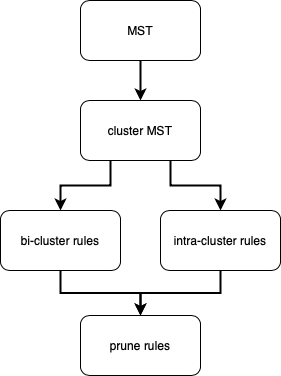
\includegraphics[scale=0.35]{ruleflow}
\caption{\algo\ algorithm}
\label{fig:algorithm_flow}
\end{figure}

%\section{Dataset Pre-Processing}
%The dataset used in this study is the sales data of $4,152,919$ transactions from a chain of Brazilian gas-station stores \pcite{data_source}.
%Each row in the dataset represents the purchase of a specific product as part of a transaction - and as such, each row corresponds to the following columns:
%\begin{itemize}
%\item Company Code
%\item Order Number
%\item Employee
%\item Product
%\item Product Category
%\item Client
%\item Sale Date Time
%\item Product Cost
%\item Discount Amount
%\end{itemize}
%All personal and corporate names were exchanged for fictitious names by the author of the dataset in order to preserve the anonymity of those whose who could have otherwise been identified through the dataset.
%% columns_to_export = ['product', 'product_category', 'client_city', 'discount_amount', 'basket_id']
%Only the Product, Product Category, Client City and Discount Amount columns were retained for the purposes of our algorithm, the rest were discarded.
%Before employing the dataset, sanitary procedures were carried out to ensure that the dataset was error-free and in a format suitable for graph generation. The steps have been detailed below.
%
%\begin{enumerate}
%\item \textbf{Transaction Identifier}\\
%The \textit{Order Number} field showed discrepancies, where a given order number could reference distinct transactions in different stores and cities, and at different dates and times. 
%This could be due to the stores maintaining their own order numbers, and also because the order numbers may reset after a predetermined limit.
%A unique transaction identifier - named \texttt{basket\_id} - was created by concatenating the order number and the date, thereby mitigating the occurrence of a identifier that references multiple transactions.
%
%\item \textbf{Binary Purchase Vector transformation}\\
%The dataset was then transformed such that each transaction was represented by a binary purchase vector - as described in Section \ref{sec:binary_purchase_vectors} - wherein each column represents a product category. The product categories were chosen for the graph representation over the products themselves as it would give a more generalized view on the associations between them, and the categories themselves were deemed specific enough that they would not be parent to children of significant variance.
%
%\end{enumerate} 
%\section{MST Generation}
%\begin{figure}[H]
%\centering
%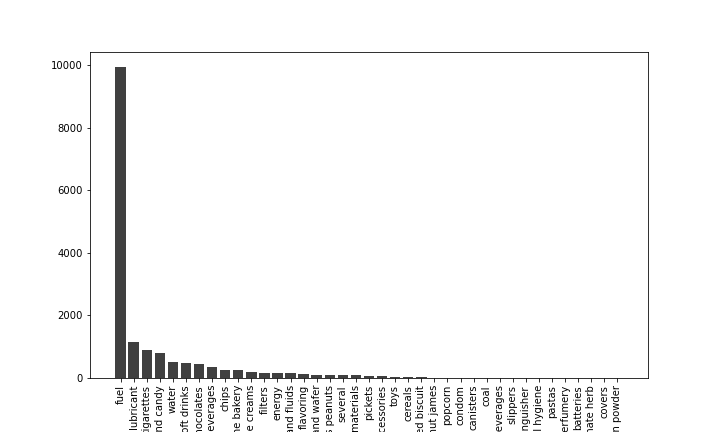
\includegraphics[scale=0.5]{category_dist}
%\caption{Category Distribution}
%\label{fig:cat_dist}
%\end{figure}
%The metrics used to assess the association rules - support, lift and confidence - are based on the proportional presence of a given itemset in the transactions. Since our dataset is from a gas-station store chain, fuel products dominate the transactional presence by a significant factor. Figure \ref{fig:cat_dist} highlights the disparity between the presence of \textit{fuel} products and the others, with \textit{fuel} being present in $99.28\%$ of all transactions. To avoid the association rules being dominated by the \textit{fuel} category - which should inherently understood to be a key product for gas stations - the fuel category was purged from the dataset, reducing the dataset to $1,362,617$ transactions.
%
%
%Following the methodology described in Section \ref{sec:binary_purchase_vectors}, a correlation matrix was computed from the binary purchase vectors using the Pearson's Correlation Coefficient. Since the correlations are of binary variables again, the correlation score is equivalent to the Phi-Coefficient $\phi$. Figure \ref{fig:correlation} illustrates the correlation matrix. Only the values below the diagonal have been illustrated as the matrix is diagonally symmetrical.
%
%
%
%
%
%\begin{figure}[H]
%\centering
%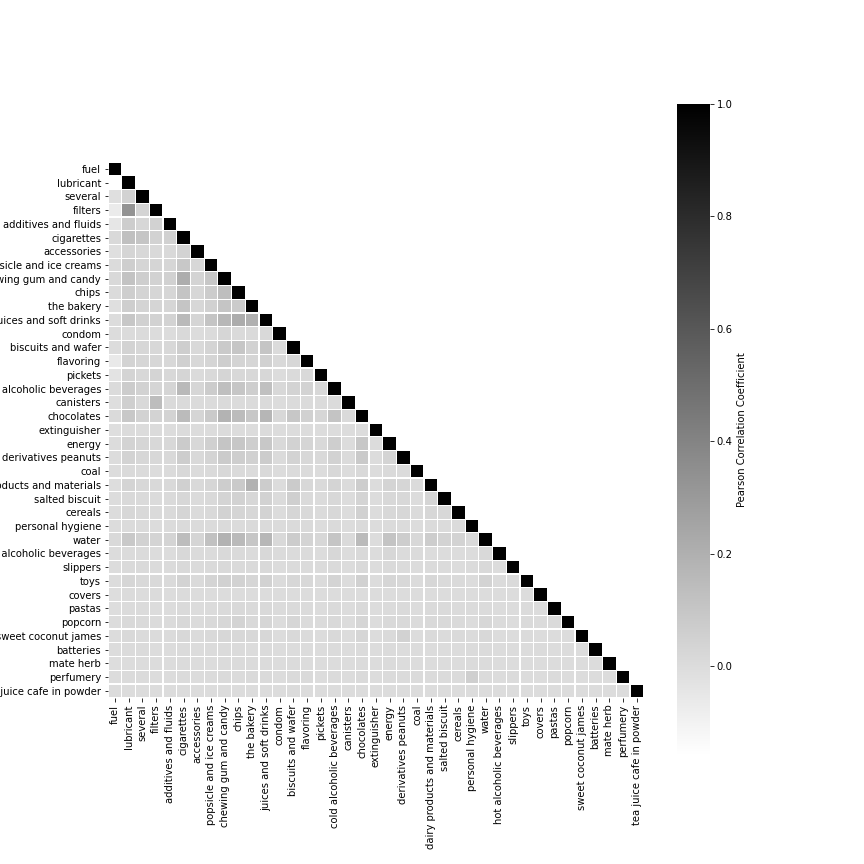
\includegraphics[scale=0.4]{correlation}
%\caption{Correlation Matrix from Binary Purchase Vectors}
%\label{fig:correlation}
%\end{figure}
%
%A minimum spanning tree is a graph composed of the \textit{shortest} path connecting all vertices, and therefore the values in the correlation matrix would need to be transformed via a function such that the higher the correlation value, the lower the output value. This would allow the MST to capture the strongest associations between the product categories. As used by \textbf{M. A. Valle et al.} in \pcite{mst_paper}, the distance function (Equation \ref{eq:distance_function}  was used to make this transformation - where $\phi_{ij}$ refers to the correlation value for two given product categories $i$ and $j$ in Figure \ref{fig:correlation}). However, whereas \textbf{M. A. Valle et al.} left their $\phi_{ij}$ unaltered, we have converted it to an absolute value (i.e. $|\phi_{ij}|$). The reason behind this is to capture the strongest relationships between product categories, positive and negative alike. By leaving the value unaltered, the MST would not capture strong negative associations as they would have the highest weights after the distance function was applied. Figure \ref{fig:distance_function} illustrates the effect of this function, where the stronger the correlation, the lower the distance function's output. The figure also demonstrates that because the Pearson's Correlation Coefficient is bound to the interval $[-1,1]$, the distance function's output is therefore bound to the interval $[0,\sqrt{2}]$. 
%\begin{equation}
%\label{eq:distance_function}
%d_{ij} = \sqrt{2(1-|\phi_{ij}|)}
%\end{equation}
%
%\begin{figure}[H]
%\centering
%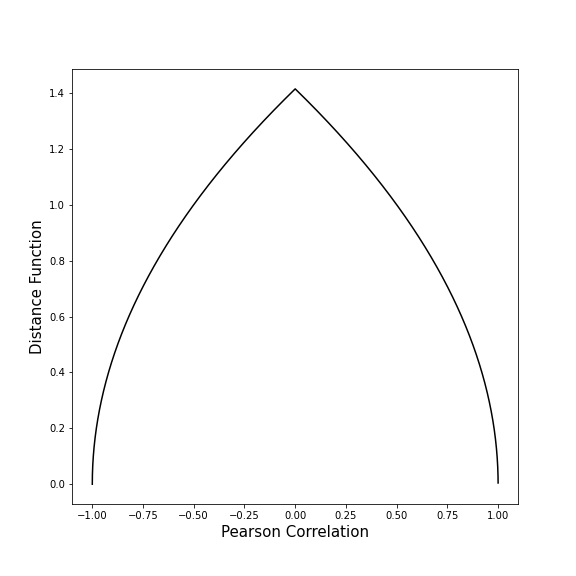
\includegraphics[scale=0.4]{distance_function}
%\label{fig:distance_function}
%\caption{The effect of the distance function $\sqrt{2(1-|x|)}$}
%\end{figure}
%
%\begin{figure}[H]
%\centering
%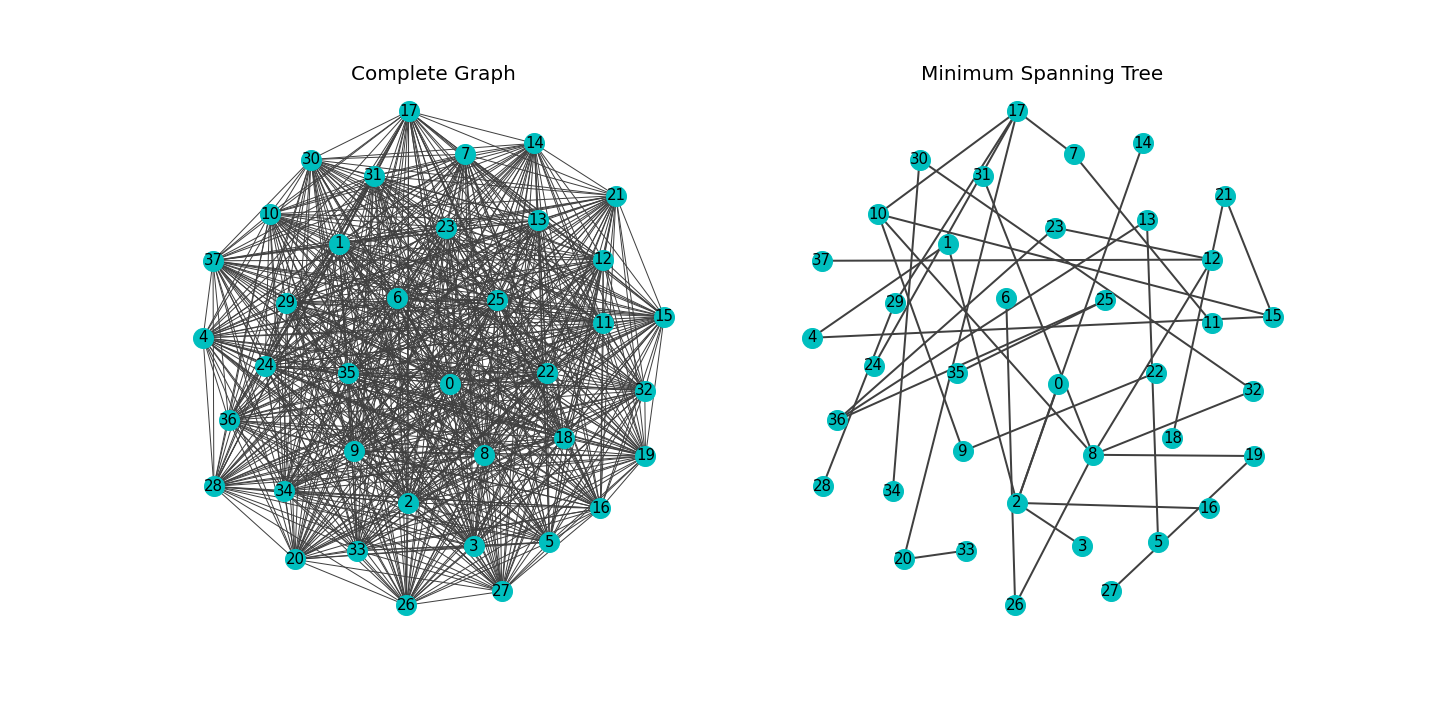
\includegraphics[scale=0.32]{graph_and_mst_no_fuel}
%\caption{Product Category Graph and MST}
%\label{fig:graph_mst}
%\end{figure}
%With the correlation matrix transformed using Equation \ref{eq:distance_function}, a graph $G = (V,E)$ was generated such that the vertices $V$ represent the product categories, and the edges $E$ the associations between them. Employing Kruskal's algorithm, a minimum spanning tree was then extracted from this graph. Both the complete graph and the MST are illustrated in Figure \ref{fig:graph_mst}. The value of each node is an integer, which corresponds with the index of the product category in the binary purchase vector dataset. The length of each edge is directly proportionate to its value, such that the greater the value, the greater the length of the edge.
%
%
%
%\section{Markov Clustering}
%The MST was then clustered using the Markov Clustering algorithm. To identify the most modular clustering configuration (modularity being the minimality of connectedness between dense clusters), an array of inflation scores between $1.5$ and $2.5$ (inclusive) were tested at increments of $0.1$, leading us to determine that an inflation score of $1.6$ resulted in the most optimal modularity. The Markov Clustering was performed using this inflation score, and the clustering results are illustrated in Figure \ref{fig:clustered} (note that while the disposition of the nodes is different from that illustrated in Figure \ref{fig:graph_mst}, the values of all nodes and edges are the same). 
%\begin{figure}[H]
%\centering
%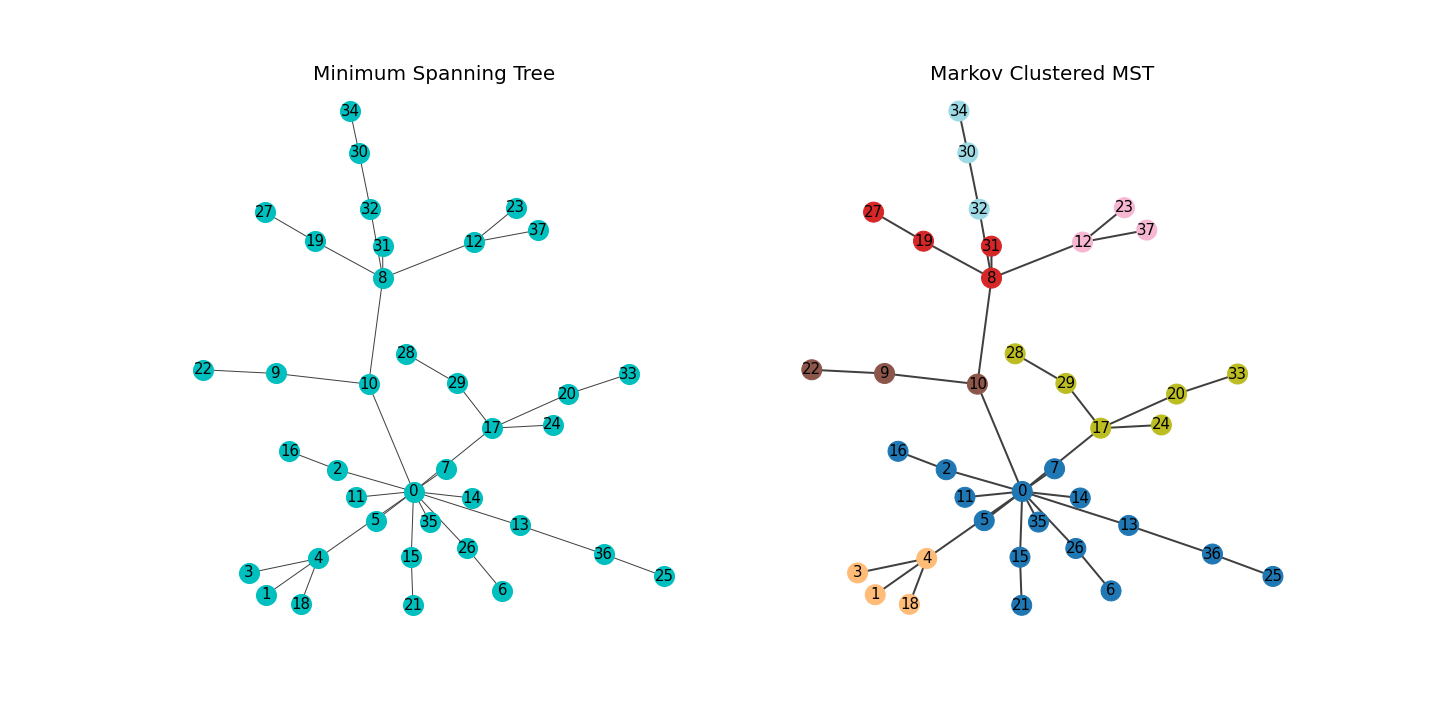
\includegraphics[scale=0.32]{mst_clustered_no_fuel2}
%\caption{MST before and after Markov Clustering}
%\label{fig:clustered}
%\end{figure}
%The Markov Clustering algorithm segmented the nodes into 8 distinct clusters.
%Figure \ref{fig:cluster_named} illustrates the names of the product categories in each cluster, color-coded in accordance with the graphs in Figure \ref{fig:clustered}.
%
%\begin{figure}[H]
%\centering
%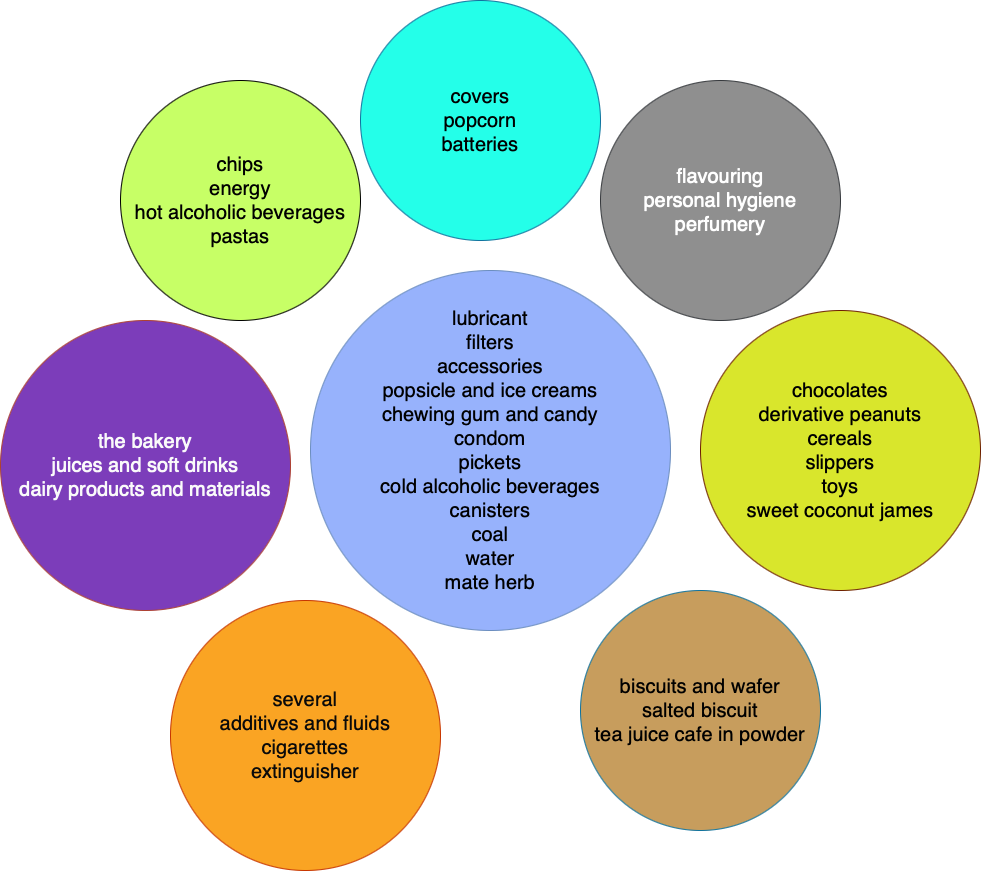
\includegraphics[scale=0.3]{cluster_named}
%\caption{Product categories by cluster}
%\label{fig:cluster_named}
%\end{figure}
%
%\section{Rule Generation}
%
%\subsection{Itemset Generation}
%For every cluster identified, all possible itemsets are generated for the $n$ product categories in a given cluster such that the length of the itemsets range from $1$ to $n-1$. Listing \ref{lst:itemset_generation} is the pseudo-code that generates all possible itemsets for a cluster.
%
%%\begin{lstlisting}[language=Python, caption=Cluster Itemset Generation, label=lst:itemset_generation]
%%# Source: arm_cython.pyx
%%from itertools import combinations
%%...
%%cpdef __generate_itemsets_by_cluster():
%%    global itemsets_by_cluster
%%    cdef set items
%%    for index, cluster in enumerate(clusters):
%%        items = set()
%%        for set_size in range(1, len(cluster)):
%%            items.update(combinations(cluster, set_size))
%%        itemsets_by_cluster[index] = items
%%\end{lstlisting}
%
%
%\begin{lstlisting}[language=C, mathescape=true, caption=Cluster Itemset Generation, label=lst:itemset_generation]
%define itemsets_by_cluster as {$\emptyset$}
%define CLUSTERS as {$c_1, c_2,\dots,c_n$}
%function generate_itemsets_by_cluster
%	for i in {$1,2,\dots,n$}
%        define items as $\emptyset$
%        // Cluster at index i
%        define cluster as CLUSTERS at i
%        for j in {$1,2,\dots,n-1$}
%            to items add all $^nC_j$ combinations of j elements from cluster
%        // Add items to items_by_cluster with cluster index as key
%        // e.g. {2: {(1,4),(2)...}}
%        to items_by_cluster add cluster_index at items
%\end{lstlisting}
%Once the minimum spanning tree has been successfully clustered, association rules can be generated from the clusters in two distinct ways.
%\subsection{Bi-Cluster Rule Generation}
%Bi-cluster rules are those where the antecedent and consequent originate from distinct and separate clusters. All possible bi-cluster permutations $^nP_2$ are calculated for $n$ clusters. Possible association rules are then generated for these combinations of clusters.
%\begin{lstlisting}[language=C, mathescape=true, caption=Cluster Itemset Generation, label=lst:bi_cluster]
%define CLUSTERS as {$c_1, c_2,\dots,c_n$}
%define itemsets_by_cluster as {$\dots$} // populated above
%function generate_bicluster_rules
%    define rules as {}
%    // all bi-cluster combinations
%    define combinations as all $^nC_2$ combinations of {$1,2,\dots,n$} with 2 elements
%    
%    for c in combinations:
%        define antecedent_cluster as (c at 1) // first index is 1
%        define consequent_cluster as (c at 2)
%        define antecedent as (itemsets_by_cluster at antecedent_cluster)
%        define consequent as (itemsets_by_cluster at consequent_cluster)
%        for antecedent_item in antededent
%            for consequent_item in consequent
%                to rules add (antecedent_item $\rightarrow$ consequent_item)
%                to rules add (consequent_item $\rightarrow$ antecedent_item)
%\end{lstlisting}
%Listing \ref{lst:bi_cluster} is the pseudo-code used to generate all the bi-cluster rules. In the pseudo-code, we have used combinations instead of permutations to gather all bi-cluster configurations. 
%If we were to use permutations, we would have to generate each itemset $i$ for clusters $A$ and $B$ such that
%	\[i_j \rightarrow i_k\;\;\;;\;\;i_k \subset A,\;\; i_j \subset B\;\; i_k \cap i_j = \emptyset\]
%and then
%	\[i_j \rightarrow i_k\;\;\;;\;\;i_k \subset B,\;\; i_j \subset A\;\; i_k \cap i_j = \emptyset\]
%which would be the same combinations in a different configuration. Instead, by using \texttt{combinations} on line $4$ of Listing \ref{lst:bi_cluster}, only computing the $i_k \rightarrow i_j$ and then re-adding the rule to the ruleset with the antecedent and consequent swapped (line $12$), we reduces our computational time for the operation by half.
%
%\subsection{Intra-Cluster Rule Generation}
%Intra-cluster rules are those where the both antecedent and consequent originate from the same cluster. Similar to the bi-cluster rules, the intra-cluster rules used the itemsets generated via the \texttt{\_\_generate\_itemsets\_by\_cluster()} function in Listing \ref{lst:itemset_generation}, however with the constraint:
%	\[i_j \rightarrow i_k\;\;\;;\;\;i_k \subset A,\;\; i_j \subset A\;\; i_k \cap i_j = \emptyset\]
%
%\subsection{Rule Pruning}
%\begin{lstlisting}[language=C, mathescape=true, caption=Rule Prune, label=lst:prune]
%define rules as {$\dots$} // all possible association rules
%define min_support as float
%define min_confidence as float
%function prune_rules
%    define valid_rules as {$\emptyset$}
%    define below_thresold as {$\emptyset$}
%    sort rules ascending by antecedent
%    for r in rules
%        // de-structure rule
%        antecedent = r at 1 // index begins at 1
%        consequent = r at 2
%        define is_above_threshold as true
%        for itemset in below_threshold
%            if itemset $\subset$ r
%                is_above_threshold = false
%                break
%        if is_above_threshold
%            // calculate supports
%            define support_antecedent as float
%            define support_consequent as float
%            define support_r as float
%            define confidence as (support_r $\div$ support_antecedent)
%            define lift as (confidence $\div$ support_consequent)
%            
%            if support_antecedent < min_support
%                to below_threshold add support_antecedent
%                next loop
%            if support_consequent < min_support
%                to below_threshold add support_consequent
%                next loop
%            if confidence < min_confidence
%                next loop
%            
%            to valid_rules add r
%\end{lstlisting}
%As described in section \ref{sec:ais}, \textit{The Apriori Principle} states that the support of a set is - at most - equal to the support of its subsets.
%\[\text{support}(\{x,y\}) \geq \text{support}(\{x,y,z\})\]
%To take advantage of this, we first sort our rules in ascending order by the number of elements in the antecedent. When iterating through the potential rules, if either the antecedent or consequent is found to have a support score below the pre-defined minimum tolerance, the itemsets are added to a set \texttt{below\_threshold}. Any future rules iterated are then cross-checked against \texttt{below\_threshold}, 
%and if it is found that any set in \texttt{below\_threshold} is a subsset of the rule, the rule is discarded as we know that its support is below our minimum tolerance. This allows us to avoid computing the support for several rules - the time complexity of which $O(n)$ per rule at worst, thereby significantly reducing computation time. For both the \textit{bi-cluster} and \textit{intra-cluster} rule generation, the rules are pruned accordingly, and those that satisfy the thresholds specified are returned.
    % Methodology
\chapter{Implementation and Analysis}

\section{Environment}
All the code for this algorithm was written in Python \pcite{py} and Rust \pcite{rust}. Python was used to read and sanitize the initial dataset, and Rust was used to generate the binary purchase vectors. We opted to use Rust instead of Python for this task because the generation of this vectors has a time complexity of $O(N^2)$ at worst, and therefore may take an order of magnitude longer to run on a slower language such as Python. Python was used for the rest of the tasks, which included the graph generation and clustering, as well as the itemset generation and rule pruning. The following external Python libraries were used to aid development:
\begin{itemize}
\item \texttt{pandas}: Data manipulation.
\item \texttt{numpy}: Data manipulation.
\item \texttt{matplotlib}: Plotting library.
\item \texttt{seaborn}: Plotting library.
\item \texttt{networkx}: Graph generation and plotting.
\item \texttt{markov\_clustering}: Markov Clustering Algorithm from \pcite{mcl_code}.
\end{itemize}

\section{Data Transformation}
\label{sec:algo_data}
Given an itemset $I = \{I_1, I_2,\dots,I_m\}$ and a set of tranactions $T = \{T_1,T_2,\dots\,T_n\}$ such that $T_i \subseteq I$, every transaction $T_i$ will be transformed into a binary purchase vector, as described in Section \ref{sec:binary_purchase_vectors}. An $m \times m$ correlation matrix will then be computed using the Pearson's Correlation Coefficient from the set of binary purchase vectors, composed of the correlation every item has against every other item. A graph $G = (V,E)$ will be constructed from this correlation matrix, such that the vertices $V=I$, and every edge will be the correlation value between the two items it connects. A minimum spanning tree is a sub-graph composed of the \textit{shortest} path connecting all vertices (i.e. the lowest sum of weights), and therefore if we construct our graph from the correlation matrix, the MST would only capture strongly negative and weakly positive relationships only, whereas we want to capture the strongest relationships between products, both negative and positive. Therefore to extract a MST with the strongest associations, the values in the correlation matrix must first be transformed before a graph is constructed from them.

\section{Distance Function}
\label{sec:distance}
As mentioned in Section \ref{sec:binary_purchase_vectors}, the Pearson's Correlation Coefficient is equivalent to the Phi Coefficient ($\phi$) for binary variables, as is the case for our binary purchase vectors. Given $\phi_{ij}$ for items $I_i$ and $I_j$ in the correlation matrix, \pcite{mst_paper} used the distance function
\[
\phi_{ij} = \sqrt{2(1-\phi_{ij})}
\]
to transform their correlation matrix. Given that we are using the Pearson's Correlation Coefficient that gives us a correlation score in the interval [-1,1], this equation is not suitable for us as it discards the strongly negative associations by outputting a larger weight (e.g. a correlation score of -1 would be transformed to 2) which would not be captured in the MST. Therefore, we modify the equation to be
\[
\phi_{ij} = \sqrt{2(1-|\phi_{ij}|)}
\]
allowing us to capture both positive and negative associations alike. Figure \ref{fig:distance_function} illustrates the effect of our distance function, where the stronger the correlation of the input, the lower the output. Given that our initial correlation values were bound to the interval $[-1,1]$, the output of the distance function is similarly bound to the interval $[0, \sqrt{2}]$.
\begin{figure}[H]
\centering
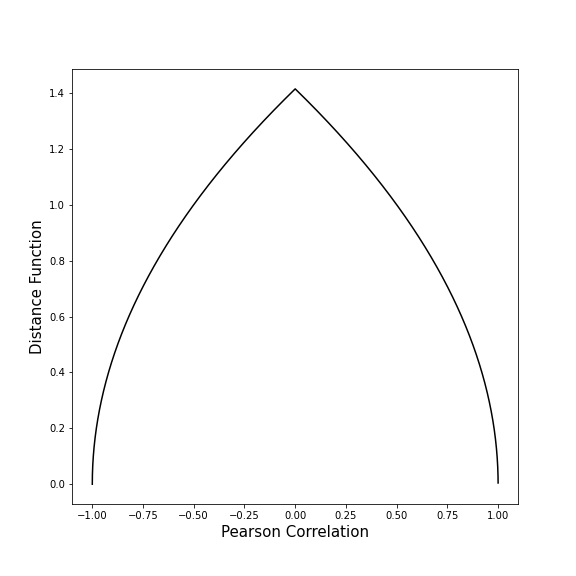
\includegraphics[scale=0.4]{distance_function}
\label{fig:distance_function}
\caption{The effect of the distance function $\sqrt{2(1-|x|)}$}
\end{figure}
\noindent Once the correlation matrix has been transformed via this function, the graph $G=(V,E)$ can be constructed with the transformed data as the weights.



\section{Dataset Pre-Processing}
The dataset used in this study is the sales data of $4,152,919$ transactions and $39$ unique product categories from a chain of Brazilian gas-station stores \pcite{data_source}.
Each row in the dataset represents the purchase of a specific product as part of a transaction - and as such, each row corresponds to the following columns:
\begin{itemize}
\item Company Code
\item Order Number
\item Employee
\item Product
\item Product Category
\item Client
\item Sale Date Time
\item Product Cost
\item Discount Amount
\end{itemize}
All personal and corporate names were exchanged for fictitious names by the author of the dataset in order to preserve the anonymity of those whose who could have otherwise been identified through the dataset.
% columns_to_export = ['product', 'product_category', 'client_city', 'discount_amount', 'basket_id']
Only the Product, Product Category, Client City and Discount Amount columns were retained for the purposes of our algorithm, the rest were discarded.
Before employing the dataset, sanitary procedures were carried out to ensure that the dataset was error-free and in a format suitable for graph generation. The steps have been detailed below.

\begin{enumerate}
\item \textbf{Transaction Identifier}\\
The \textit{Order Number} field showed discrepancies, where a given order number could reference distinct transactions in different stores and cities, and at different dates and times. 
This could be due to the stores maintaining their own order numbers, and also because the order numbers may reset after a predetermined limit.
A unique transaction identifier - named \texttt{basket\_id} - was created by concatenating the order number and the date, thereby mitigating the occurrence of a identifier that references multiple transactions.

\item \textbf{Binary Purchase Vector transformation}\\
The dataset was then transformed such that each transaction was represented by a binary purchase vector - as described in Section \ref{sec:algo_data} - wherein each column represents a product category. The product categories were chosen for the graph representation over the products themselves as it would give a more generalized view of the associations\footnote{as supported by \pcite{market_ass} in Section \ref{sec:subjective}}, and the categories themselves were deemed specific enough that they would not be parent to children of significant variance.
\end{enumerate} 
\begin{figure}[H]
\centering
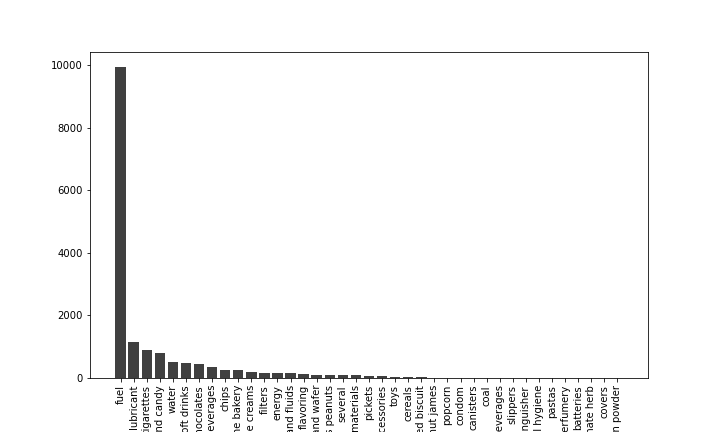
\includegraphics[scale=0.5]{category_dist}
\caption{Category Distribution}
\label{fig:cat_dist}
\end{figure}
The metrics used to assess the association rules - support, lift and confidence - are based on the proportional presence of a given itemset in the transactions. Since our dataset is from a gas-station store chain, fuel products dominate the transactional presence by a significant factor. Figure \ref{fig:cat_dist} highlights the disparity between the presence of \textit{fuel} products and the others, with \textit{fuel} being present in $99.28\%$ of all transactions. To avoid the association rules being dominated by the \textit{fuel} category - which should inherently understood to be a key product for gas stations - the fuel category was purged from the dataset, reducing the dataset to $1,362,617$ transactions.
The correlation matrix for the $38$ remaining product categories was then computed using Pearson's Correlation Coefficient, and is illustrated in Figure \ref{fig:correlation}. Since the correlation matrix is known to be diagonally symmetrical, only the values below the diagonal have been illustrated.
\begin{figure}[H]
\centering
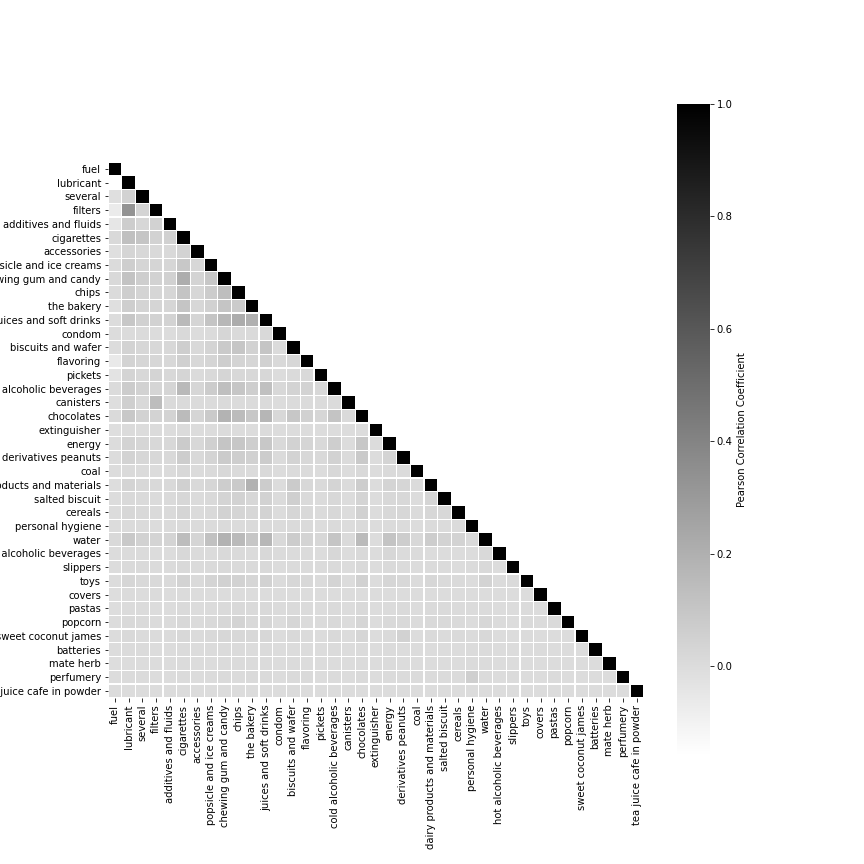
\includegraphics[scale=0.4]{correlation}
\caption{Correlation Matrix from Binary Purchase Vectors}
\label{fig:correlation}
\end{figure}


\section{MST Generation}
As described in \ref{sec:distance}, the distance function $\sqrt{2(1-|\phi_{ij}|)}$ was then applied to the correlation matrix to transform the values such that the strongest associations have the lowest values. The graph $G=(V,E)$ was then constructed such that the vertices $V$ represent the product categories, and the weights of the edges $E$ are the transformed correlation values between the vertices the edges connect. The minimum spanning tree was then extracted from this graph using Kruskal's algorithm. Both the complete graph and the MST are illustrated in Figure \ref{fig:graph_mst}. The value of each node is an integer, which corresponds to the index of the product category in the binary purchase vector dataset. The length of each edge is directly proportionate to its weight, such that the greater the weight, the greater the length of the edge.
\begin{figure}[H]
\centering
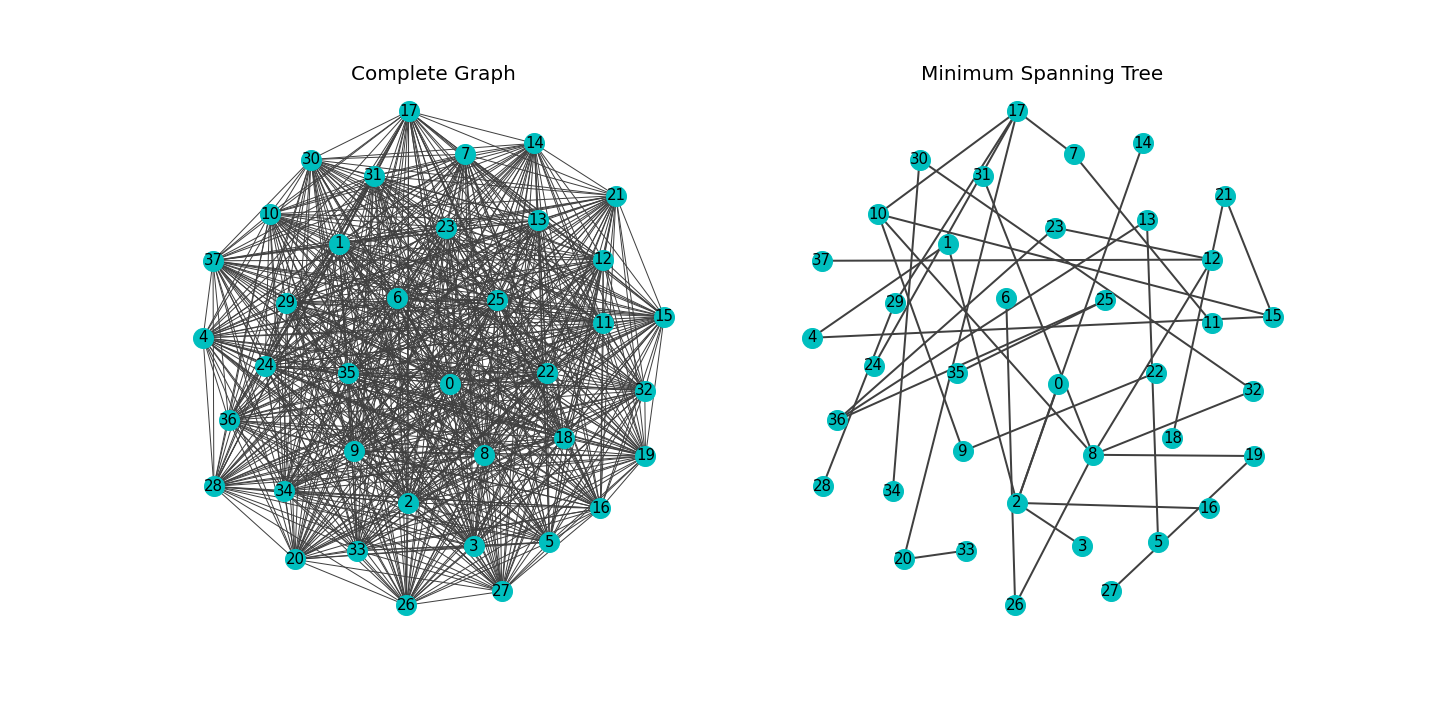
\includegraphics[scale=0.31]{graph_and_mst_no_fuel}
\caption{Product Category Graph and MST}
\label{fig:graph_mst}
\end{figure}

\section{Markov Clustering}
\begin{figure}[H]
\centering
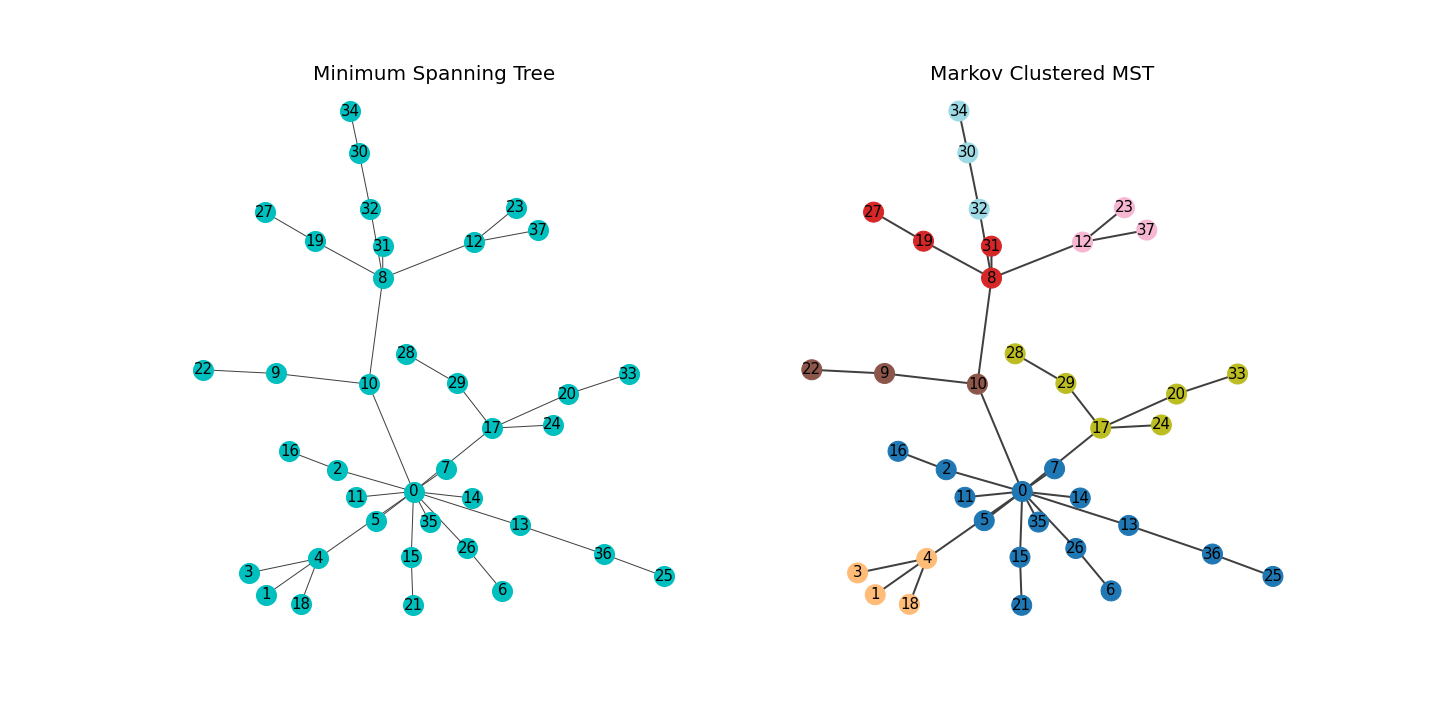
\includegraphics[scale=0.31]{mst_clustered_no_fuel2}
\caption{MST before and after Markov Clustering}
\label{fig:clustered}
\end{figure}
The MST was then clustered using the Markov Clustering (MCL) algorithm. To identify the most modular clustering configuration, we implemented the MCL algorithm several times with inflation scores between 1.5 and 2.5 (inclusive) at increments of 0.1. In doing so, we discovered that an inflation score of 1.6 resulted in the most optimal modularity. The Markov Clustering configuration produced using this inflation score was therefore chosen, and the results of this clustering are illustrated in Figure \ref{fig:clustered}. Note that while the disposition of nodes differs from that illustrated in Figure \ref{fig:graph_mst}, the nodes and the edge weights are the same.
The Markov Clustering algorithm segmented the nodes into 8 distinct clusters.
Figure \ref{fig:cluster_named} illustrates the names of the product categories in each cluster, color-coded in accordance with the MSTs in Figure \ref{fig:clustered}. Observing the groupings produced by the MCL algorithm, we can see that with the exception of the largest cluster in blue, the groupings do have an underlying similarity (e.g. \texttt{\{biscuits and wafer, salted biscuit, tea juice cafe in powder\}}).

\begin{figure}[H]
\centering
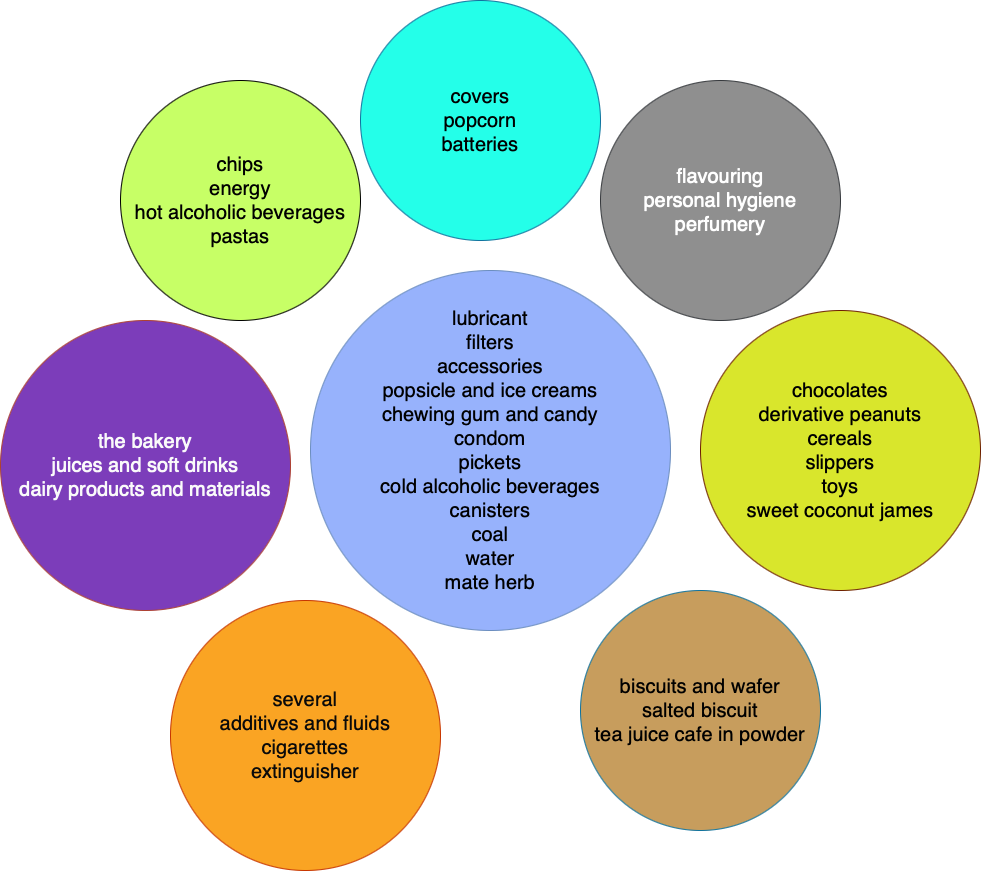
\includegraphics[scale=0.3]{cluster_named}
\caption{Product categories by cluster}
\label{fig:cluster_named}
\end{figure}


\section{Comparison of \algo\ and Apriori Algorithm}
Once the MST was clustered, we used both the \algo\ and the Apriori Algorithm to generate rules for our dataset, with the support constraint at $0.1\%$ and the confidence constraint at $25\%$. Given these constraints, the Apriori algorithm generated $1,222$ rules, and the \algo\ generated $123$ bi-cluster rules as well as $60$ intra-cluster rules, totalling $183$ rules.\\
\\\\\textbf{Apriori Rules}\\
We present the first 5 rules generated by the Apriori Algorithm, ranked by highest support.

\begin{longtable}
{@{}llllll@{}}\toprule Antecedent& Consequent& Support& Confidence& Lift& Type\\*\midrule\endfirsthead\endhead
\{chewing gum and candy\} & \{cigarettes\} & 0.0726 & 0.2986 & 1.0985 & Apriori\\
\{cigarettes\} & \{chewing gum and candy\} & 0.0726 & 0.2671 & 1.0985 & Apriori\\
\{water\} & \{chewing gum and candy\} & 0.0473 & 0.3052 & 1.2554 & Apriori\\
\{filters\} & \{lubricant\} & 0.0468 & 0.9381 & 2.6850 & Apriori\\
\{chocolates\} & \{chewing gum and candy\} & 0.0435 & 0.3117 & 1.2820 & Apriori\\
\midrule\caption{Apriori Rules}\label{tab:apri_rules}\end{longtable}

\noindent \textbf{\algo\ Rules}\\
Similarly, we present the first 5 rules generated by the \algo, ranked by highest support. The type of rule has also been annotated (i.e. bi-cluster or intra-cluster).

\begin{longtable}
{@{}llllll@{}}\toprule Antecedent& Consequent& Support& Confidence& Lift& Type\\*\midrule\endfirsthead\endhead
\{chewing gum and candy\} & \{cigarettes\} & 0.0726 & 0.2986 & 1.0985 & bi-cluster\\
\{cigarettes\} & \{chewing gum and candy\} & 0.0726 & 0.2671 & 1.0985 & bi-cluster\\
\{water\} & \{chewing gum and candy\} & 0.0473 & 0.3052 & 1.2554 & intra-cluster\\
\{filters\} & \{lubricant\} & 0.0468 & 0.9381 & 2.6850 & intra-cluster\\
\{chocolates\} & \{chewing gum and candy\} & 0.0435 & 0.3117 & 1.2820 & bi-cluster\\
\midrule\caption{\algo\ rules}\label{tab:arm_rules}\end{longtable}

\noindent \textbf{Analysis}\\
We observe that there is a $100\%$ overlap between the top five rules generated by the Apriori algorithm and the \algo. The $100\%$ overlap stands true for up until the first $13$ rules for both algorithms, after which a decline can be observed. 
\begin{figure}[H]
\centering
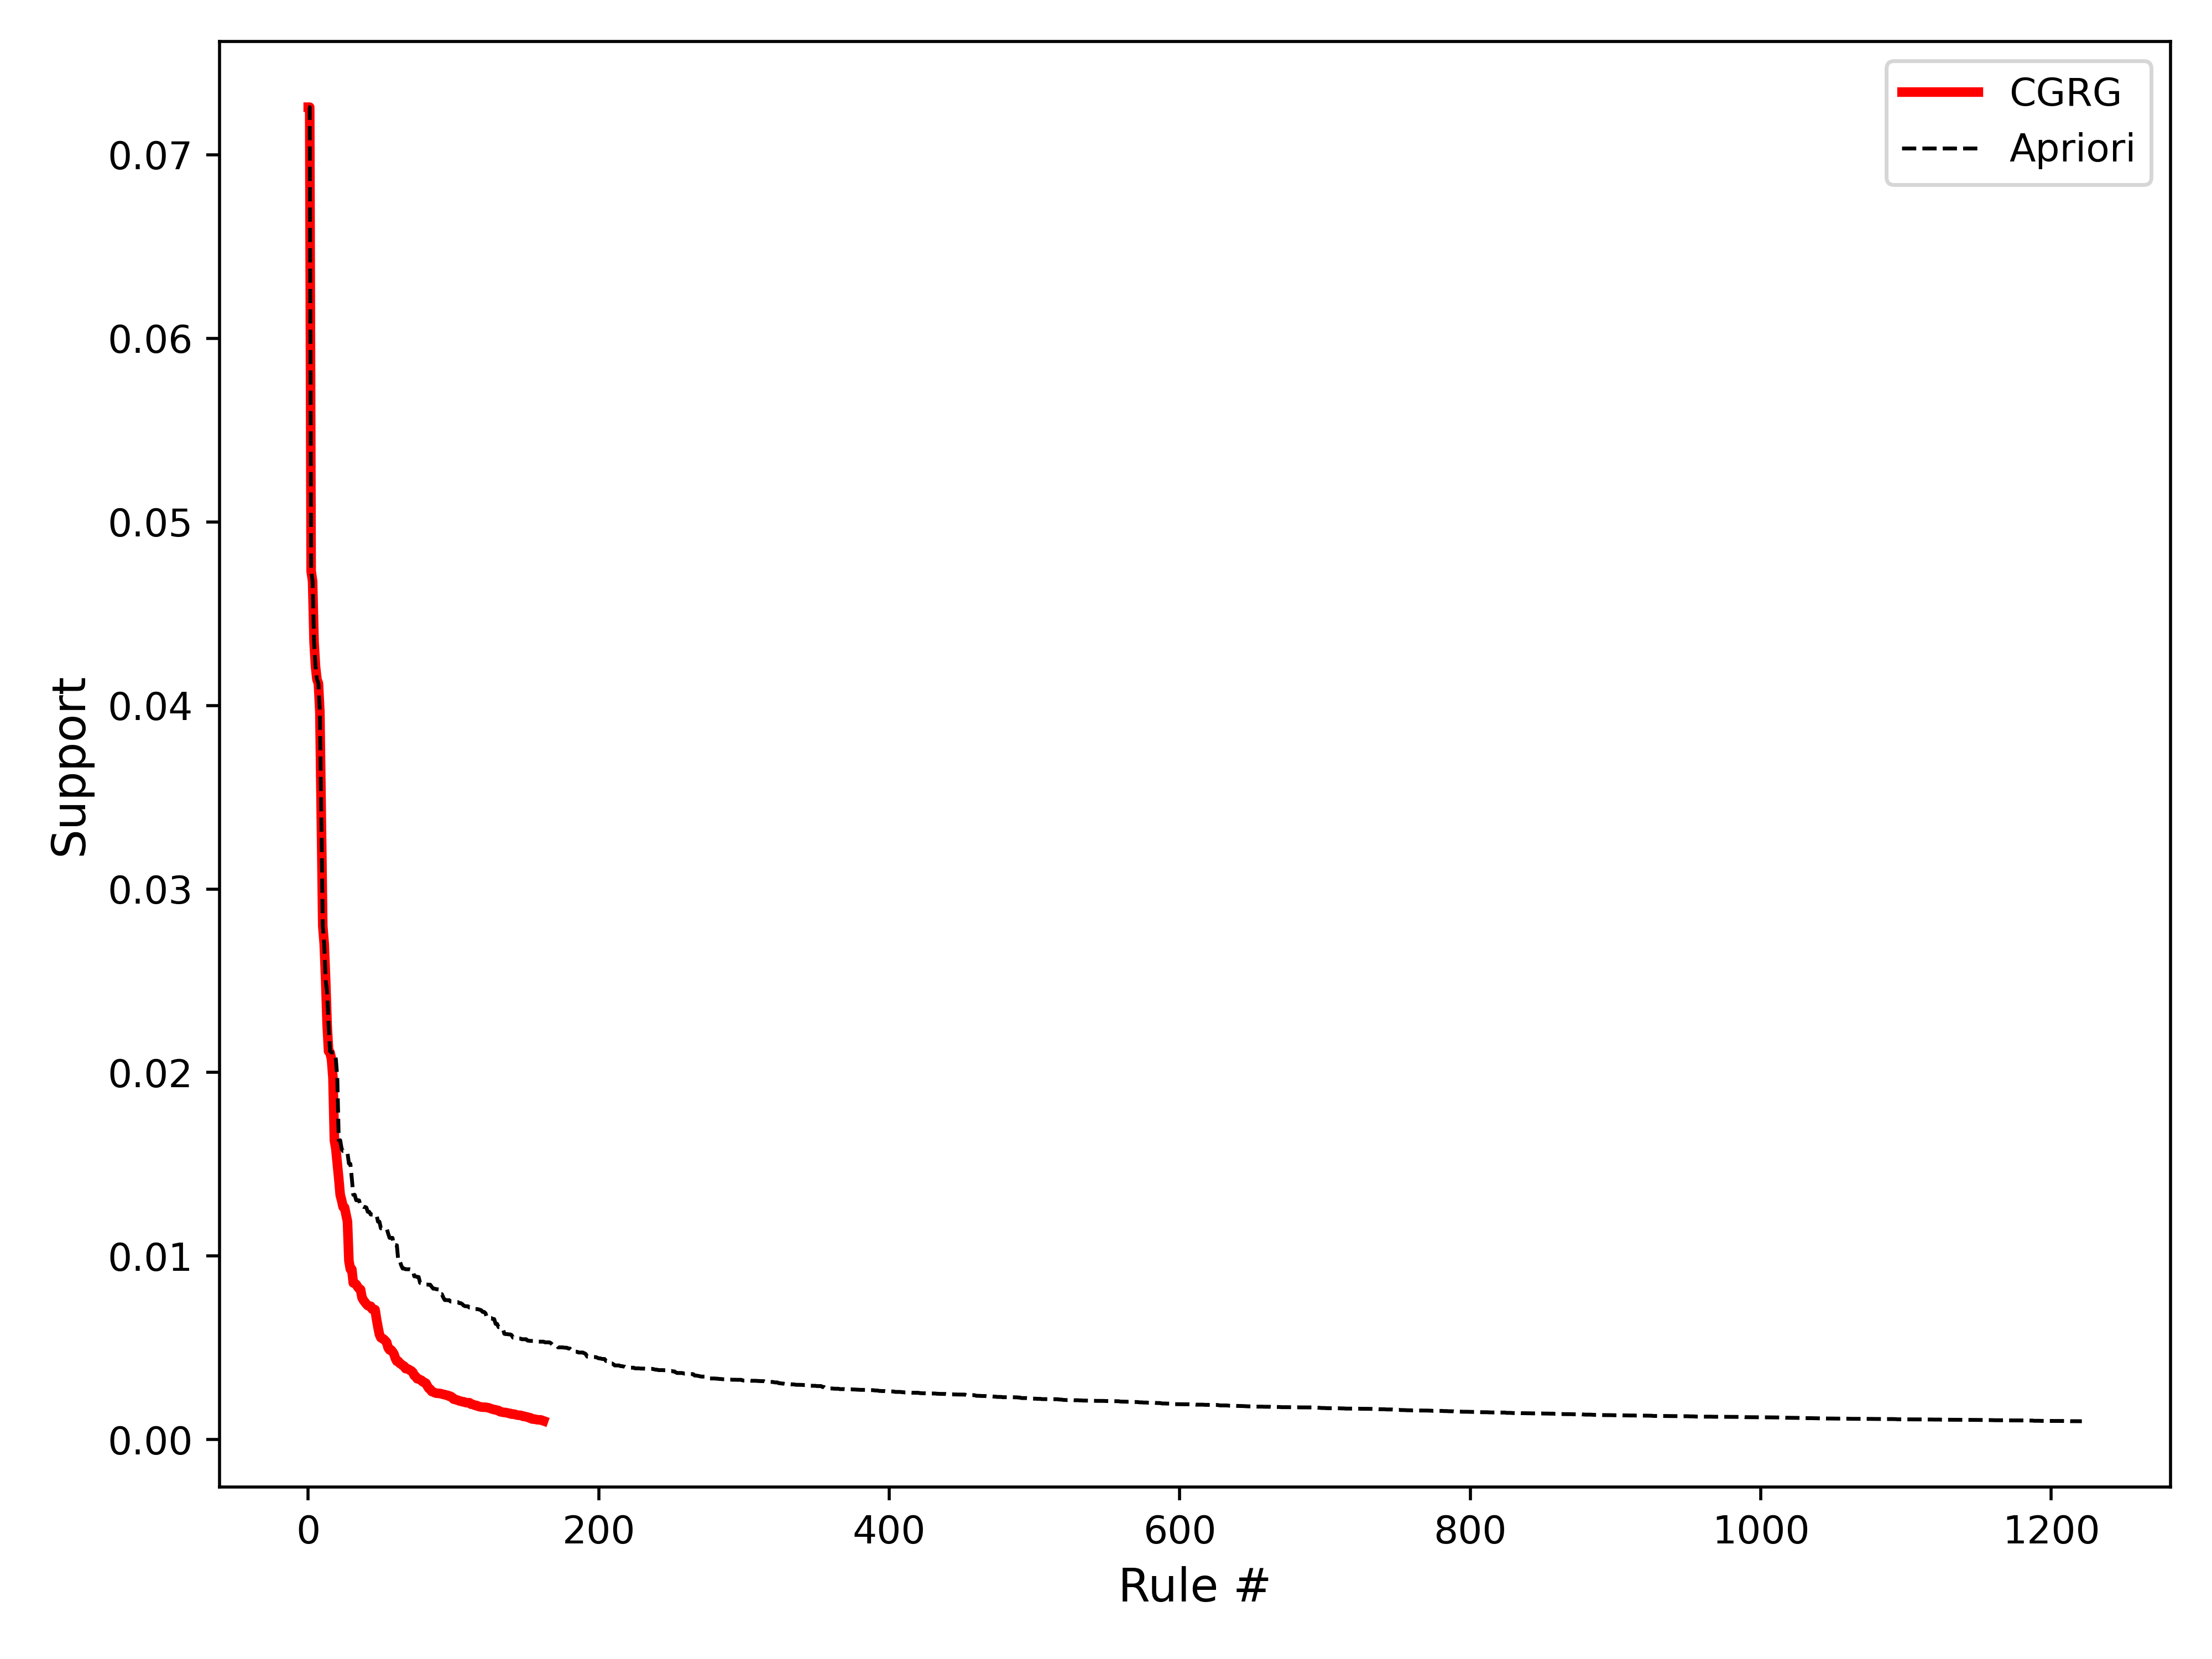
\includegraphics[scale=0.65]{ruleset_support}
\caption{Ranked supports for both the \algo\ and Apriori Algorithm}
\label{fig:rule_support}
\end{figure}
\noindent Figure \ref{fig:rule_support} illustrates the support values for the $x^{th}$ rule for both the \algo\ and Apriori when they are sorted by the highest support score to the lowest. 
We can observe that when provided with the same support and confidence constraints, the Apriori algorithm produces far greater rules, whereas the \algo\ algorithm captures mostly the those rules that have a relatively higher support, with the exception being at the elbow of both curves, where the \algo\ algorithm captured rules with a lower support than the Apriori algorithm.\\
We can infer from this figure that the \algo\ algorithm captures the strongest rules present in the Apriori ruleset, which leads us to theorize that \textit{rules where the itemsets each originate from the same cluster are likelier to have a higher support score than those which don't}. In other words, given clusters $A$ and $B$, and subsets of any given cluster $cl_i$ and $cl_j$, rules which follow:
\[
cl_i \rightarrow cl_j;\;\;\;cl_i \subset A, \;\;\; (cl_j \subset B \;|\; cl_j \subset A)
\]
are likelier to have a higher support score than rules whose antecedent and/or consequent are composed of items from multiple clusters.
To further reinforce this theory, we present the averages of the support, confidence and lift scores generated by both algorithms:
\begin{longtable}
{@{}llll@{}}\toprule Algorithm& Mean Support& Mean Confidence& Mean Lift\\*\midrule\endfirsthead\endhead
Apriori & 0.0034& 0.3737& 1.9096\\
\algo\ & 0.0075& 0.3683& 1.8855\\
\midrule\caption{Averages for both algorithms}\end{longtable}
\noindent We can see that while the mean confidence and lift scores from the Apriori algorithm are only marginally higher those from the \algo\ algorithm, the mean support for the \algo\ algorithm is significantly greater than that of the Apriori algorithm by a factor of approximately $2.2$, indicating that the composition of the rules generated by the \algo\ algorithm is far more concentric in high-value rules than the Apriori generated ruleset. This is contradicted to a degree by the lack of mid-value rules in the \algo\ ruleset that were present in the Apriori ruleset at the elbow of the curve in Figure \ref{fig:rule_support}.
\begin{figure}[H]
\centering
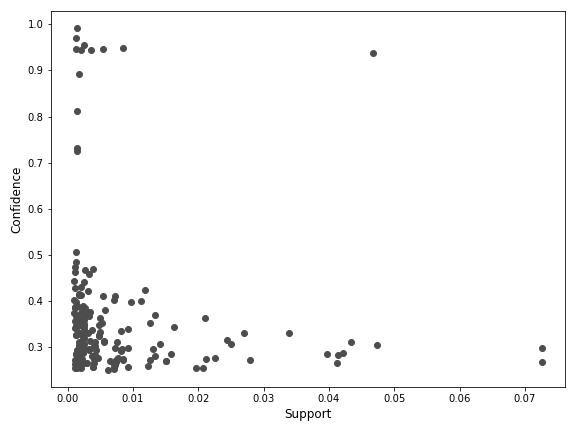
\includegraphics[scale=0.65]{confsupp}
\caption{Relationship between confidence and support for \algo}
\label{fig:confsupp}
\end{figure}
Figure \ref{fig:confsupp} illustrates the relationship between the confidence and support for the rules generated by the \algo\ algorithm.
The majority of rules generated are concentric around the support and confidence constraints of $0.001$ and $0.25$ respectively. The outliers indicate a negative relationship between the two metrics: the rules with the highest confidence had a relatively low support, and vice versa.

As \pcite{lift} argued, the \textit{lift} score may be a better metric to assess the value of a rule than support or confidence. Figure \ref{fig:rule_lift} illustrates the lift values for the $x^{th}$ rule for both the \algo\ and Apriori when they are sorted by the highest lift score to the lowest. The image has been zoomed to illustrate only the first $183$ rules (the length of the \algo\ ruleset) to further illustrate the disparity at the elbows of the curves.
\begin{figure}[H]
\centering
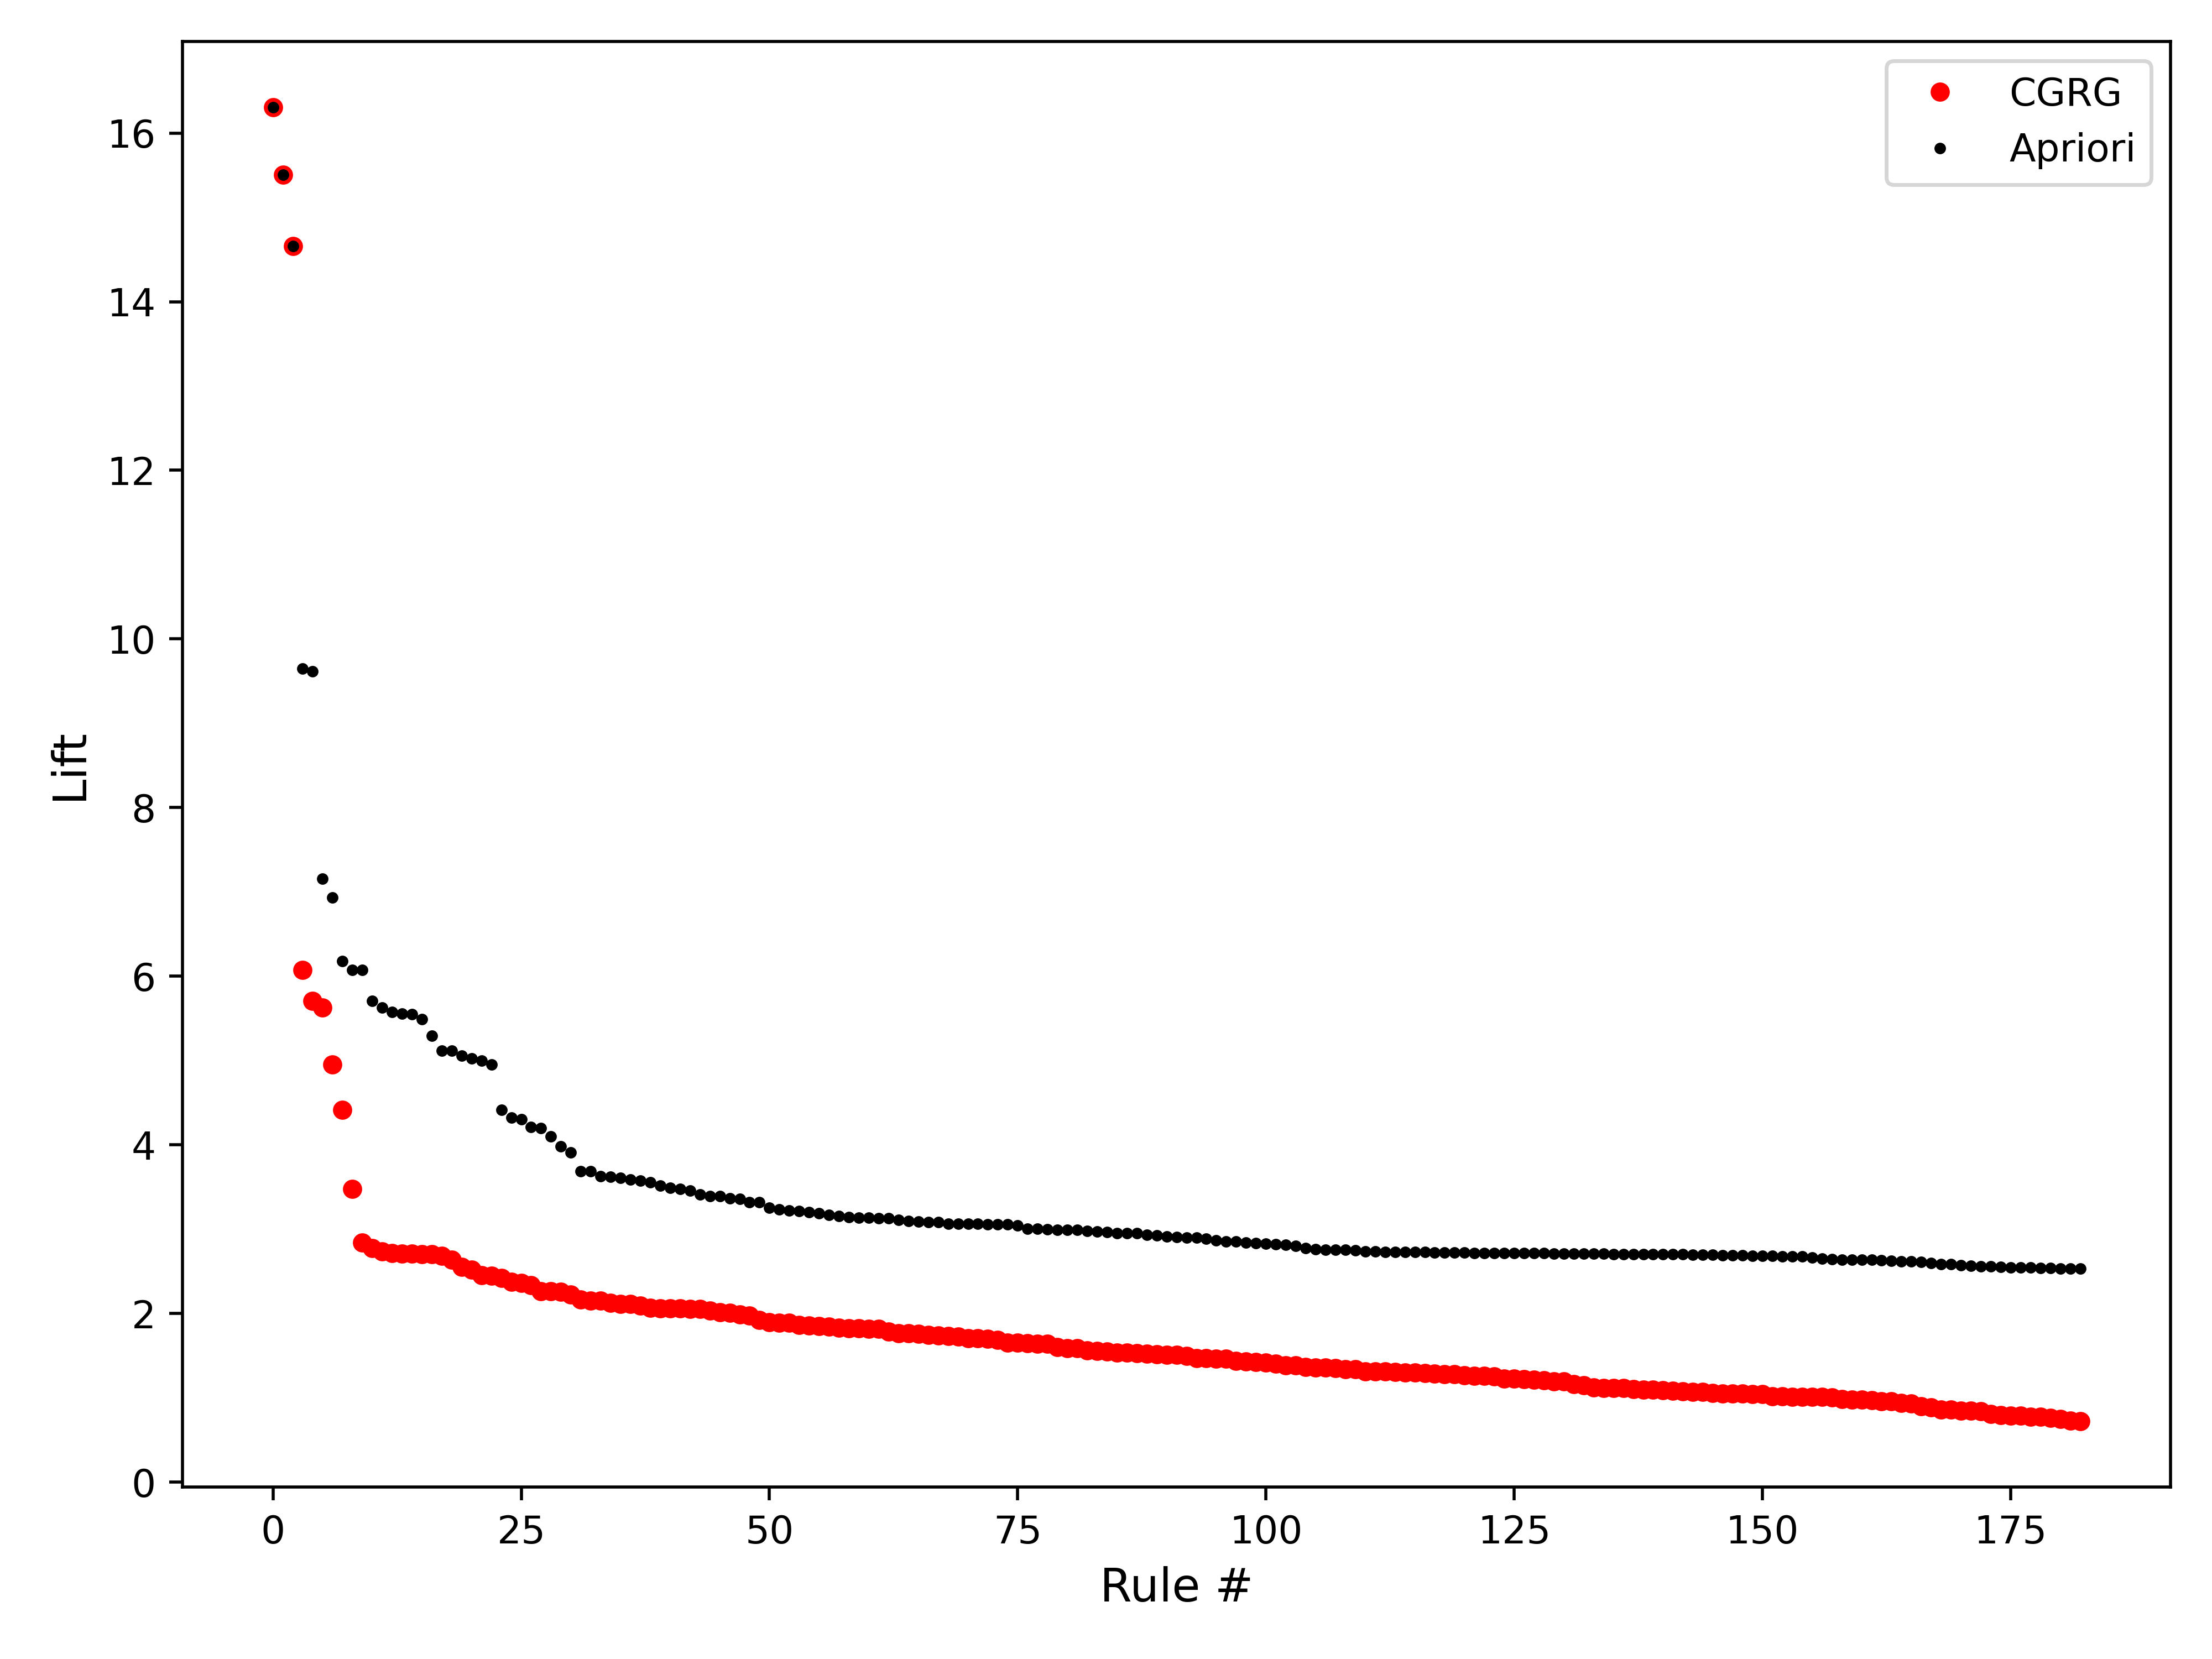
\includegraphics[scale=0.65]{ruleset_lift_zoom}
\caption{Ranked lift scores for both the \algo\ and Apriori Algorithm}
\label{fig:rule_lift}
\end{figure}
The figure is similar to the ranked support scores in Figure \ref{fig:rule_support}, however the disparity at the elbow of the curves is much greater. This may indicate that the antecedent may give a higher rise to the confidence of a rule when the composition of the antecedent and/or the consequent consists of items from multiple clusters. To illustrate the high lift rules our algorithm has failed to capture, the first five rules generated by both algorithms and ranked by lift scores have been detailed below:

\begin{longtable}
{@{}llllll@{}}\toprule Antecedent& Consequent& Support& Confidence& Lift& Type\\*\midrule\endfirsthead\endhead
\{canisters,lubricant\} & \{filters\} & 0.0014 & 0.8128 & 16.3071 & Apriori\\
\{canisters\} & \{filters,lubricant\} & 0.0014 & 0.7250 & 15.5054 & Apriori\\
\{canisters\} & \{filters\} & 0.0014 & 0.7308 & 14.6611 & Apriori\\
\{chips,filters\} & \{juices and soft drinks,lubricant\} & 0.0011 & 0.3528 & 9.6487 & Apriori\\
\{filters,the bakery\} & \{juices and soft drinks,lubricant\} & 0.0011 & 0.3515 & 9.6143 & Apriori\\
\midrule\caption{Apriori Rules ranked by Lift}\label{tab:apri_lift}\end{longtable}

\begin{longtable}
{@{}llllll@{}}\toprule Antecedent& Consequent& Support& Confidence& Lift& Type\\*\midrule\endfirsthead\endhead
\{lubricant,canisters\} & \{filters\} & 0.0014 & 0.8128 & 16.3071 & intra-cluster\\
\{canisters\} & \{lubricant,filters\} & 0.0014 & 0.7250 & 15.5054 & intra-cluster\\
\{canisters\} & \{filters\} & 0.0014 & 0.7308 & 14.6611 & intra-cluster\\
\{filters,water\} & \{lubricant,chewing gum and candy\} & 0.0020 & 0.3525 & 6.0734 & intra-cluster\\
\{lubricant,pickets\} & \{filters\} & 0.0013 & 0.2844 & 5.7052 & intra-cluster\\
\midrule\caption{\algo\ Rules ranked by Lift}\end{longtable}
The first three rules with the highest lift are present in the rulesets of both algorithms, however the \algo\ did not capture the fourth and fifth rule in Table \ref{tab:apri_lift}. This further reinforces our belief that the structural constraints of the rules the \algo\ algorithm produces impedes the algorithm from generating the rules such as those present in the Table \ref{tab:apri_lift}. We can therefore conclude that while the \algo\ algorithm produces a smaller albeit higher value ruleset compared to the Apriori algorithm, it also fails to generate the mid-value rules that were present in the Apriori algorithm.     % Results and Experiments
\chapter{Conclusions}
\section{Achievements}
In this paper, we have introduced a new algorithm for association rule generation - the \algo\ algorithm: an extension of the methodology proposed by \pcite{mst_paper} that also employs the techniques and principles outlined in \pcite{apriori} and \pcite{markov_clustering}. The \algo\ algorithm produces bi-cluster rules where the antecedent and consequent are from separate clusters, and intra-cluster rules where both the antecedent and consequent originate from the same cluster. In doing so, it appears to capture the high-support rules from all possible rules within any support and confidence constraints.  We have also theorized that association rules that are bi-cluster or intra-cluster tend to have a higher support score than those rules that are not. The rules generated by the \algo\ algorithm seem to also follow general intuition (see: Table \ref{tab:arm_rules}) such as \texttt{\{cigarettes\}} $\rightarrow$ \texttt{\{chewing gum and candy\}}, and \texttt{\{filters\}} $\rightarrow$ \texttt{\{lubricant}\}, further reinforced by their existence in the rules generated by the Apriori algorithm as well.

\section{Limitations}
\textbf{Dataset Bias}\\
All analysis was conducted on the topological structures generated from a singular dataset. This may not be wholly representative of the rules the \algo\ algorithm may generate, and perhaps a different dataset may have yielded different results.
\\\textbf{Clustering}\\
As seen in Figure \ref{fig:cluster_named} on Page \pageref{fig:cluster_named}, the Markov Clustering configuration yielded some clusters that seem appropriate, yet some (for example, the largest) were perhaps too broad to classify under a single cluster.
\\\textbf{Rule Structure}\\
The \algo\ algorithm's key feature is both its greatest strength and drawback. Due to the fact that our algorithm only selects those rules where the items in a given itemset are from the same cluster, the algorithm overlooks rules where the antecedent and consequent have a composition of items from multiple clusters. 
Figures \ref{fig:rule_support} and \ref{fig:rule_lift} indicate that the \algo\ algorithm did not generate several higher-value rules present at the elbow of the Apriori rule curve.
However, we have also concluded via Figure \ref{fig:rule_support} that this constraint captures a majority of high-value (i.e. high support) rules and does not capture the lower-value rules within the support and confidence constraints.


\section{Future Works}
As mentioned, a key limitation of our analysis is that it only applies to the dataset we used. Future projects involving different datasets may produce new insights into the advantages and/or limitations of the algorithm. Additionally, alternative clustering algorithms may be considered as a replacement for the Markov Clustering algorithm. 
  % Conclusions

% ----------------------------------------------------------
% Do not write below this line
% ----------------------------------------------------------
% References
\renewcommand*{\mkbibnamefamily}[1]{\textsc{\textbf{#1}}}
\renewcommand*{\mkbibnameprefix}[1]{\textsc{\textbf{#1}}}
\renewcommand*{\mkbibnamegiven}[1]{\textsc{\textbf{#1}}}
\renewcommand*{\mkbibnamesuffix}[1]{\textsc{\textbf{#1}}}
\printbibliography[heading=bibintoc, title=References]

% ------------------------------------------------------------------------------
% End document
% ------------------------------------------------------------------------------
\end{document}
